\documentclass[11pt,a4paper,twoside,openright]{Thesis}
\usepackage[T1]{fontenc}
\usepackage[utf8]{inputenc}
\usepackage[english]{babel}
\usepackage{verbatim}
\usepackage{float}
\usepackage{textcomp}
\usepackage{booktabs}
\usepackage{array}
\usepackage{amsthm}
\usepackage{amstext}
\usepackage{amsmath}
\usepackage{amssymb}
\usepackage{graphicx}
\usepackage{xcolor}
\usepackage{tikz}
\usepackage{mathtools}

\usetikzlibrary{arrows,automata,shapes,positioning,fit}
\usepackage{algpseudocode}
\usepackage{float}
\usepackage{caption}
\usepackage{algorithm}
\algnewcommand{\LineComment}[1]{\State \(\triangleright\) #1}

\DeclarePairedDelimiter\floor{\lfloor}{\rfloor}

\theoremstyle{definition}
\newtheorem*{notation}{Notation}
\newtheorem*{defn}{Definition}
\newtheorem{thm}{Theorem}

% ============================================================
%% Uncomment the next few lines to get sf URL links:
%\usepackage{url}
%\makeatletter
%\def\url@leostyle{%
%  \@ifundefined{selectfont}{\def\UrlFont{\sf}}{\def\UrlFont{\small\sffamily}}}
%\makeatother
%\urlstyle{leo} % Now actually use the newly defined style.
%% Choose coloured or b/w links:
% \usepackage{hyperref}
% ============================================================
% Markup macros for proof-reading
\usepackage{ifthen}
\usepackage[normalem]{ulem} % for \sout
\usepackage{xcolor}
\newcommand{\ra}{$\rightarrow$}
\newboolean{showedits}
\setboolean{showedits}{false} % toggle to show or hide edits

\newcommand{\Figref}[1]{figure~\ref{fig:#1}}
\newcommand{\Secref}[1]{section~\ref{sec:#1}}
\newcommand{\Tabref}[1]{table~\ref{tab:#1}}
\newcommand{\figlabel}[1]{\label{fig:#1}}
\newcommand{\seclabel}[1]{\label{sec:#1}}
\newcommand{\tablabel}[1]{\label{tab:#1}}

\hypersetup{pdftitle={\ttitle}}
\hypersetup{pdfsubject=\subjectname}
\hypersetup{pdfauthor=\authornames}
\hypersetup{pdfkeywords=\keywordnames}

\newcommand{\nes}[1]{\textcolor{red}{#1}}
\ifthenelse{\boolean{showedits}}
{
	\newcommand{\ugh}[1]{\textcolor{red}{\uwave{#1}}} % please rephrase
	\newcommand{\ins}[1]{\textcolor{blue}{\uline{#1}}} % please insert
	\newcommand{\del}[1]{\textcolor{red}{\sout{#1}}} % please delete
	\newcommand{\chg}[2]{\textcolor{red}{\sout{#1}}{\ra}\textcolor{blue}{\uline{#2}}} % please change
}{
	\newcommand{\ugh}[1]{#1} % please rephrase
	\newcommand{\ins}[1]{#1} % please insert
	\newcommand{\del}[1]{} % please delete
	\newcommand{\chg}[2]{#2}
}
% ============================================================
% Put edit comments in a really ugly standout display
%\usepackage{ifthen}
\usepackage{amssymb}
\newboolean{showcomments}
\setboolean{showcomments}{true}
%\setboolean{showcomments}{false}
\newcommand{\id}[1]{$-$Id: scgPaper.tex 32478 2010-04-29 09:11:32Z oscar $-$}
\newcommand{\yellowbox}[1]{\fcolorbox{gray}{yellow}{\bfseries\sffamily\scriptsize#1}}
\newcommand{\triangles}[1]{{\sf\small$\blacktriangleright$\textit{#1}$\blacktriangleleft$}}
\ifthenelse{\boolean{showcomments}}
%{\newcommand{\nb}[2]{{\yellowbox{#1}\triangles{#2}}}
{\newcommand{\nbc}[3]{
 {\colorbox{#3}{\bfseries\sffamily\scriptsize\textcolor{white}{#1}}}
 {\textcolor{#3}{\sf\small$\blacktriangleright$\textit{#2}$\blacktriangleleft$}}}
 \newcommand{\version}{\emph{\scriptsize\id}}}
{\newcommand{\nbc}[3]{}
 \renewcommand{\ugh}[1]{#1} % please rephrase
 \renewcommand{\ins}[1]{#1} % please insert
 \renewcommand{\del}[1]{} % please delete
 \renewcommand{\chg}[2]{#2} % please change
 \newcommand{\version}{}}
\newcommand{\nb}[2]{\nbc{#1}{#2}{orange}}
\newcommand{\here}{\yellowbox{$\Rightarrow$ CONTINUE HERE $\Leftarrow$}}
\newcommand\rev[2]{\nb{TODO (rev #1)}{#2}} % reviewer comments
\newcommand\fix[1]{\nb{FIX}{#1}}
\newcommand\todo[1]{\nb{TO DO}{#1}}
\newcommand\on[1]{\nbc{ON}{#1}{red}} % add more author macros here
\newcommand\ml[1]{\nbc{ML}{#1}{violet}} % add more author macros here
%\newcommand\XXX[1]{\nbc{XXX}{#1}{blue}}
%\newcommand\XXX[1]{\nbc{XXX}{#1}{brown}}
%\newcommand\XXX[1]{\nbc{XXX}{#1}{cyan}}
%\newcommand\XXX[1]{\nbc{XXX}{#1}{darkgray}}
%\newcommand\XXX[1]{\nbc{XXX}{#1}{gray}}
%\newcommand\XXX[1]{\nbc{XXX}{#1}{magenta}}
%\newcommand\XXX[1]{\nbc{XXX}{#1}{olive}}
%\newcommand\XXX[1]{\nbc{XXX}{#1}{orange}}
%\newcommand\XXX[1]{\nbc{XXX}{#1}{purple}}
%\newcommand\XXX[1]{\nbc{XXX}{#1}{red}}
%\newcommand\XXX[1]{\nbc{XXX}{#1}{teal}}
%\newcommand\XXX[1]{\nbc{XXX}{#1}{violet}}
% ============================================================


% Alter some LaTeX defaults for better treatment of figures:
    % See p.105 of "TeX Unbound" for suggested values.
    % See pp. 199-200 of Lamport's "LaTeX" book for details.
    %   General parameters, for ALL pages:
    \renewcommand{\topfraction}{0.9}	% max fraction of floats at top
    \renewcommand{\bottomfraction}{0.8}	% max fraction of floats at bottom
    %   Parameters for TEXT pages (not float pages):
    \setcounter{topnumber}{2}
    \setcounter{bottomnumber}{2}
    \setcounter{totalnumber}{4}     % 2 may work better
    \setcounter{dbltopnumber}{2}    % for 2-column pages
    \renewcommand{\dbltopfraction}{0.9}	% fit big float above 2-col. text
    \renewcommand{\textfraction}{0.07}	% allow minimal text w. figs
    %   Parameters for FLOAT pages (not text pages):
    \renewcommand{\floatpagefraction}{0.7}	% require fuller float pages
	% N.B.: floatpagefraction MUST be less than topfraction !!
    \renewcommand{\dblfloatpagefraction}{0.7}	% require fuller float pages

	% remember to use [htp] or [htpb] for placement


\newcommand{\pos}{\mathbf{\mathbf{p}}}
\author{Aaron Karper \and Niko Schwarz}
\begin{document}
\special{papersize=8.5in,11in}
\setlength{\pdfpageheight}{\paperheight}
\setlength{\pdfpagewidth}{\paperwidth}

\newcommand{\abs}[1]{\left|#1\right|}

\frenchspacing

\title{Efficient regular expressions that produce parse trees}

\maketitle

\begin{abstract}
Regular expressions naturally and intuitively define parse trees that describe
the text that they're parsing.  We describe a technique for building up the
complete parse tree resulting from matching a text against a regular
expression.

In previous tagged deterministic finite-state automaton (TDFA) matching
implementations, all paths through the non-deterministic finite-state automaton
(NFA) are walked simultaneously, in different co-routines, where inside each
co-routine, it is fully known when which capture group was entered or left. We
extend this model to keep track of not just the last opening and closing of
capture groups, but all of them. We do this by storing in every co-routine a
history of the all groups using the flyweight pattern. Thus, we log enough
information during parsing to build up the complete parse tree after matching
in a single pass, making it possible to use our algorithm with strings
exceeding the machine's memory. Further we construct the automata such that a
simulation of backtracking like behaviour is possible. This is achieved in
worst case time $\Theta(m\,n)$, providing full parse trees with only constant
slowdown compared to matching.
\end{abstract}

\tableofcontents

\chapter{Introduction}

Regular expressions give us a concise language to describe patterns in
strings and can be used for log analysis, natural language processing, and
many other tasks involving structured data in strings. Their efficiency make
them useful even for large data sets. Standard algorithms run in
$\mathcal{n\, m}$, where $n$ is the length of the string to be matched
against and $m$ is the length of the pattern\cite{Sedg90a}.

A short-coming of standard regular expression engines is that they can
extract only a limited amount of information from the string. A regular
expression can easily describe that a text matches a comma separated values
file, but it is unable to extract all the values.  Instead it only gives a
single instance of values:

\texttt{((.*?),(\textbackslash d+);)+} might describe a dataset of ASCII names
with their numeric label. Matching the regular expression on \texttt{``Tom
Lehrer,1;Alan Turing,2;''} confirms that the list is well formed, but the
match contains only \texttt{``Tom Lehrer''} for the second capture group
and \texttt{``1''} for the third. That is, the parse tree found by the
\textsc{Posix} is seen in \Figref{posix}.

\begin{figure}[htp]
\centering
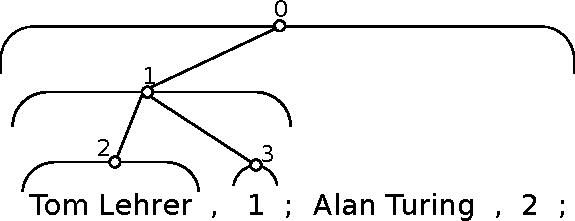
\includegraphics[width=.75\linewidth]{graphs/posix_parse}
\caption[Posix parse tree]{\figlabel{lehrer-posix} Parse tree produced by
\textsc{Posix}-compatible matching \texttt{((.*?),(\textbackslash d+);)+}
against input ``Tom Lehrer,1;Alan Turing,2;''.}
\figlabel{posix}
\end{figure}

With our algorithm we are able to reconstruct the full parse
tree after the matching phase is done, as seen in \Figref{our-tree}.

\begin{figure}[htp]
\centering
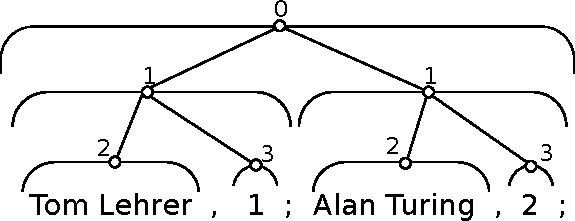
\includegraphics[width=.75\linewidth]{graphs/full_parse}
\caption[Full parse tree]{\figlabel{lehrer-tree} Parse tree produced by our approach matching
regular expression \texttt{((.*?),(\textbackslash d+);)+} against input ``Tom
Lehrer,1;Alan Turing,2;''}
\figlabel{our-tree}
\end{figure}

The worst-case run time of our approach is $\Theta(n\,m)$, the same as the
algorithm extracting only single matches. It is the first algorithm to achieve
this bound, while extracting parse trees.

\section{More powerful than standard regular expressions}
\seclabel{power}
It may at first seem as if all capture groups can always, equivalently,
be extracted by splitting the input, and then applying sub-regular
expressions on the splits.  This is, for example, an entirely valid
strategy to extract the parse tree in \Figref{lehrer-tree}.  However,
this can quickly become an exercise of writing an entire parser,
using no regular expression engine at all, even if the underlying
grammar is entirely regular.  The following grammar is hard to parse
using a regular expression engine, even though it is regular.

Consider a file of semicolon-terminated records, each record consisting
of a comma-separated pair of entries, and each entry can be escaped
to contain semicolons, as in the regular expression
\texttt{((".*?"|[a-z]*),(".*?"|[a-z]*);)+}. Here, expression
\texttt{.*?} is a non-greedy match which will be discussed in more
detail in \Secref{algo}.  This language contains, for example, the
string: ``"h;i",there;"h;,i",Paul;''.  It is easy to see that, in
order to extract all four capture group matches, it is insufficient
to split the input at the semicolon, as that would split the field
``h;i'' in half.  More involved examples, where hand-written parsers
become harder to make and more inefficient, are easily constructed.
In contrast, our approach yields the entire parse tree, simply from
the regular expression in at most $O(n\,m)$ time.

\section{Motivation}

A first step of processing large data sets is often to parse strings in order
to obtain a more manageable format. As an example, consider log files.  As
Jacobs\cite{Jaco09a} noted, ``What makes most big data big is repeated
observations over time and/ or space,'' and thus log files grow large
frequently. At the same time, they provide important insight into the process
that they are logging, so their parsing and understanding is important.

Regular expressions make for scalable and efficient lightweight parsers\cite{Kart96a}.

The parsing abilities of regular expression have provoked Meiners to declare
that for intrusion detection, ``fast and scalable RE matching is
now a core network security issue.'' \cite{Mein10a}

For example, Arasu et al. \cite{Aras12a} demonstrate how regular
expressions are used in Bing to validate data, by checking whether
the names of digital cameras in their database are valid.

Parsers that can return abstract syntax trees are more useful than
ones that only give a flat list of matches. Of course only regular
grammars can be matched by our approach.

\section{Regular expressions}
Before we dive into the algorithm to match regular expressions, we should
first look at the goal -- what regular expressions are and what kind of
constructs need to be supported by our algorithm.

Regular expressions have some constructs specific to them and literal
character matches. They are typically described in a string describing the pattern.
They can describe any regular language\cite{Sips05a} if one only
considers \emph{match} vs \emph{non-match} though they are typically used to
extract information.

\begin{table}[htb]
  \begin{tabular}{c|c|c|>{\centering\arraybackslash}m{5cm}}
    Name & Example & Repetitions & Description \\
    \hline
    literal & \texttt{a} & 1 & \\
    character ranges & \texttt{[a-z]} & 1 & any of the characters in the range
                                            match \\
    negated character ranges & \texttt{[\string^a-z]} & 1 & anything except for the
    characters in the range match \\
    \hline
    \texttt{?} operator & \texttt{a?} & 0 or 1 & \\
    \texttt{*} operator & \texttt{a*} & $0-\infty$ & Prefer more matched \\
    \texttt{+} operator & \texttt{a+} & $1-\infty$ & \\
    \hline
    \texttt{??} operator & \texttt{a??} & 0 or 1 & \\
    \texttt{*?} operator & \texttt{a*?} & $0-\infty$ & Prefer less matched \\
    \texttt{+?} operator & \texttt{a+?} & $1-\infty$ & \\
    \hline
    alternation operator & \texttt{a|b} & 1 & match one or the other, prefer left \\
    \hline
    capture groups & \texttt{(a)} & 1 & treat pattern as single element,
    extract match \\
  \end{tabular}
  \caption{Summary of regular expression elements}
\end{table}

\paragraph{Literals} The simplest option are literal characters like
\texttt{a}.

\paragraph{Character ranges} Instead of matching only a single character, a
regular expression might match any of a range of characters. This is denoted
with brackets. For example \texttt{[a-z]} would match any lowercase ASCII
letter, \texttt{[abc]} would only match the letters a, b, or c, and
\texttt{[a-gk-t]} would match any letter between a and g, or between k and t.
There is also the special character range \texttt{.} that matches any character.

\paragraph{Negated character ranges} Ranges of the form \texttt{[\string^\dots]}
negate their content, so \texttt{[\string^a-g]} would match anything except a through g.

\paragraph{Concatenation} Two constructs put after each other have to match
the string in order. For example \texttt{a[bc]} matches a followed by either
b or c.

\paragraph{Option operator} The option operator denoted by \texttt{?} allows
either zero or one repetitions of the preceding element, preferring to have
one repetition. This means \texttt{a?} will match the empty string or $a$, but nothing else.

\paragraph{Star operator} The star operator \texttt{*} allows for arbitrary
repetition of the preceding element, including zero repetitions, preferring as
many repetitions as possible. For example \texttt{a*} matches the empty string,
``a'', ``aa'', and so on.

\paragraph{Plus operator} The plus operator \texttt{+} is similar, but
requires at least one repetition. This leads to $a+$ and $aa*$ matching the
same strings.

\paragraph{Non-greedy operators} The option, the star, and the plus operators
also have corresponding non-greedy operators, which are \texttt{??},
\texttt{*?}, and \texttt{+?} respectively. These operators prefer to match as
few repetitions as possible. In back-tracking implementation, guessing the
right path is an important efficiency feature and for all capturing
implementation the path taken influences the captured groups.

\paragraph{Alternation} Patters separated by the pipe symbol \texttt{|} can
either match the left part or the right part. This binds weaker than
concatenation. Therefore \texttt{abc|xyz} would match $abc$ or $xyz$, but not
$abxyz$.

\subsection{Capture groups}
Patterns enclosed by parens are treated as a single element, thus
\texttt{(ab)*} captures $ab$, but not $aba$. More importantly for us is that
after the match, the capture groups can be extracted: \texttt{a(b*)c} when
matching $abbbc$ can extract $bbb$ and the empty string when matching $ac$.
Note that the capture groups can be nested and the semantics differ for
\textsc{Posix} and tree regular expressions: In \textsc{Posix} the regular expression
\texttt{a((bc+)+)} on the string $abcbccc$ gives $bcbccc$ for the outer
capture group and $bc$ for the inner capture group -- the leftmost occurrence of
outer capture groups is kept and within that substring, the leftmost occurrence
of the inner group is kept. In tree regular expressions, all occurrences are kept and returned
in a tree structure: The outer capture group contains $bcbccc$ and both inner
matches $bc$ and $bccc$.

\paragraph{Greediness}
The relevance of greedy and non-greedy matches becomes apparent now: The
regular expression \texttt{a(.*)c?} on the string $abc$ captures $bc$ in
the group, while \texttt{a(.*?)c?} captures only $b$. This is because
the parsing is ambiguous without specifying the greediness of the match -- both
$b$ and $bc$ would be valid.

\section{Backtracking}\seclabel{backtracking}
An intuitive and extensible algorithm for determining whether a string
matches a regular expression is backtracking. This
algorithm~\ref{alg:match-bt} is used as is or in a more optimized form in
many languages, such as Java\footnote{\texttt{java.util.regex}},
Python\footnote{The module \texttt{re}}, or Perl\cite{Cox07a}. For all its
advantages and ease of implementation the main problem is that it takes
$\Theta(2^n\,m)$ time in the worst case:

\begin{algorithm*}
  \begin{algorithmic}
  \Function{match-bt}{string, pattern}
    \If{string and pattern empty}
      \State \Return{matches}
    \ElsIf{string or pattern empty}
      \State \Return{no match}
    \ElsIf{first element of pattern is $a\mathtt{*}$}
      \LineComment{x[1:] means removing the first element of the list}
      \If{$a$ matches first element of string}
        \State \Return{match-bt(string[1:], pattern)}
      \Else
        \State \Return{match-bt(string, pattern[1:])}
      \EndIf
    \ElsIf{\dots}
      \State \dots
    \EndIf
  \EndFunction
  \end{algorithmic}
  \caption{\label{alg:match-bt}Overview of backtracking}
\end{algorithm*}

If we have the pattern \texttt{(x*)*y} matching against the
string\footnote{$x^n$ means $x$ repeated $n$ times} $x^n$, we see that it
cannot match, but it takes exponential time doing so. In each step there
are two options, either to collect the $x$ in \texttt{x*}, or to step over it
and try again. Unfortunately that means that the algorithm branches in each
character in the string and never succeeding keeps on trying, so it takes $2^n$
steps to end in the $no\ match$ case.  Backtracking is fast if it guesses
correctly, since there is not much overhead, but fails miserably if it guesses
wrongly early on.

Because it is so intuitive we will use it as the definition of a correct 
behaviour throughout this article.

\section{(Non-)deterministic finite-state automata}
As they are heavily used throughout this paper, let us recall what
non-deterministic finite-state automata (NFA) and deterministic finite-state
automata (DFA) are. A DFA is a state machine that walks over a finite
transition graph, one step for every input character. The choice of transition
is limited by the transition's character range. A transition can only be
followed if the current input character is inside transition's character
range. The possible character ranges are assumed to be disjoint, so that in
every step at most one transition can be followed.

NFA differ from DFA in that for some input character and some state, there
may be more than one applicable transition and some transitions can be
traversed without consuming a character, called $\varepsilon$-transitions.  If
there is a transition that leads to the accepting state eventually, an NFA
finds it, by trying the alternatives in lock-step.
\autoref{fig:example-automaton} shows an example of an NFA's transition graph.

An simple way to think about the process of reading input with an NFA is that
of \emph{co-routines}. A co-routine is a procedure that has the ability to
suspend itself and continue later -- it is similar to a thread, but they
don't need to be executed in parallel. In order to resume their work later,
they contain some kind of memory that is specific to them.

In the context of NFAs, a co-routine contains the current state and has access
to the transition graph. When reading a
string, the NFA maintains a set of co-routines and advance them in
lock-step. This means that each co-routine reads the current character and
spawn new co-routines for all possible transitions. When reading a character,
a co-routine must consume it, but might follow $\varepsilon$-transitions
afterwards. In order to model that, we propose an additional state kept in
the co-routine: it can either be \emph{hungry} or \emph{fed}. If it is
hungry, it can only follow transitions that contain the character to be read,
but the co-routine becomes fed. If a co-routine is fed, it can only
follow $\varepsilon$-transitions.

Furthermore the order in which states are expanded will become relevant. For
this, the model of the NFA is expanded for allowing transitions with negative
priority. An edge with negative priority will only be expanded when there are
no more legal transitions with regular priority. The order for high and low
priorities is depth first\footnote{In an implementation this would imply that
a newly seen state is put on a stack.}.

\chapter{Related work}
\seclabel{related}
While there is no shortage of books discussing the usage of regular
expressions, the implementation side of regular expression has not
been so lucky. Cox is spot-on when he argues that innovations have
repeatedly been ignored and later reinvented \cite{Cox07a,Cox09a,Cox10a}, in 
part, not least because the publication medium of source code without
accompanying article was chosen.

Regular expressions are by no means new and originated with Kleene in the
1950ies\cite{Sips05a}. This chapter first introduces some standard
procedures for regular expression matching (without extracting any
information), such as Backtracking in \Secref{backtracking} and various
automata based approaches in sections~\ref{sec:nfa-match}, \ref{sec:dfa-match},
and \ref{sec:lazy-dfa-match}. In \Secref{tfsa} we discuss an addition to
the automata based approaches called \emph{tags} that allows for the extraction
of sub-matches. We show that backtracking based approaches are not the
straw man that one could believe them to be in \Secref{revise-backtrack}.
Even though we first believed ourselves to be, we are actually not the first
to produce parse trees in competitive time, as seen in \Secref{parse-trees-related}.

A problematic aspect of the literature is that many authors perceive regular 
expression parsing a linear problem -- linear in the length of the string 
with a constant for the pattern size. This limits the applications, because 
this means that an algorithm that takes $O(2^m+n)$ time seems very 
competitive for a fixed $m$, but is prohibitively expensive for large $m$. 
The argument that the pattern is typically small seems circular to the 
authors, because would the implementation focus on allowing large patterns, 
new applications using large patterns would arise\footnote{To check if a document
contains features $f_1, f_2, \dots, f_n$, we would match the document
against regular expression \texttt{($f_1$)|($f_2$)|$\dots$|($f_n$)}.}.

In this paper, we will consider the best known algorithms quadratic. It is 
not known if there is any algorithm that beats the $O(n\, m)$ matching, but 
in \Secref{lower-bound}, a lower bound of $\Theta(n\, \min(m, \abs{\Sigma}))$ 
is proven.

\section{NFA based matching}\label{sec:nfa-match}
A faster alternative to the backtracking approach discussed in
\Secref{backtracking} is to pre-process the regular expression and convert it
into an NFA by the rules in \Figref{thompson-construction-simple}.

\begin{figure*}[htb] 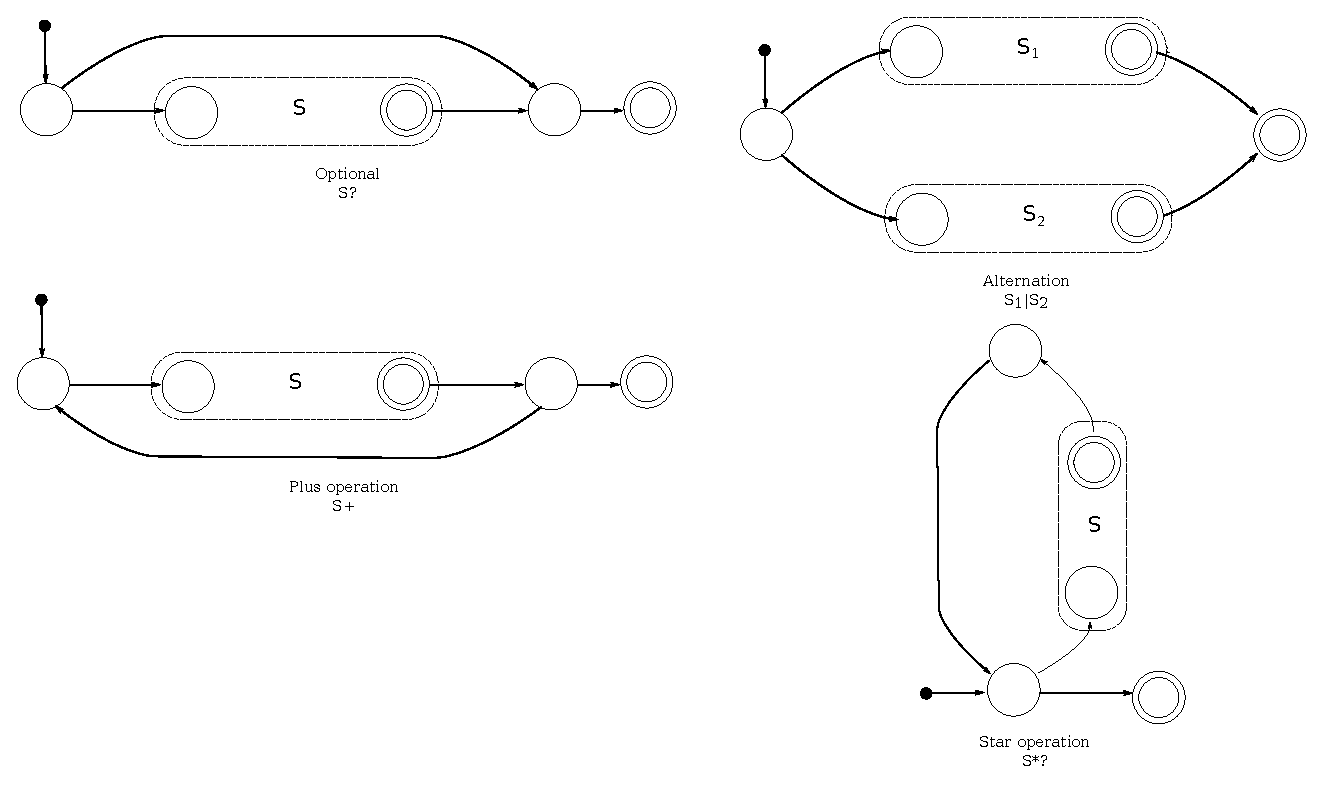
\includegraphics[width=\linewidth]{graphs/thompson-simple}
  \caption[Thompson construction]{Thompson~\cite{Thom68a} construction of the
automaton: Descend into the abstract syntax tree of the regular
expression and expand the constructs recursively.}
\label{fig:thompson-construction-simple}
\end{figure*}

The NFA thus obtained contains $O(m)$ states and to check if a given string
matches the regular expression, we can now simply run the NFA on it. For each
character in the input string, we follow all transitions possible from our
current states and save the accessible states as a set. In the next
iteration, we consider the transitions from any of these states. This allows
us to match in $O(n\, m)$ time\footnote{Note that the number of branches per 
state is $O(1)$}.

\section{DFA based matching}\label{sec:dfa-match}
Dissatisfied with the multiplicative $O(m)$ overhead, we can construct a DFA
from the NFA before matching. This is done by the power set
construction\cite{Sips05a}, which has time complexity $O(2^m)$. The idea is to
replace all states by the set reachable from it with only
$\varepsilon$-transitions. The transitions simulate a step in the original NFA,
so they point to another set of states.  After the compilation is done,
matching the string is $O(n)$ time.

This can be very useful, if the regular expression is statically known.

\section{Lazy DFA compilation}\label{sec:lazy-dfa-match}
The DFA based matching takes $O(n + 2^m)$, which is no better than backtracking
if $m$ is not fixed. The power set construction simulates every transition
possible in the NFA, but that is actually unnecessary: Instead we can
intertwining the compilation and the matching to only expand new DFA states that
are reached when parsing the string. At most one new DFA state is created after
each character read and if necessary the whole DFA is constructed, after
which the algorithm is no different from the eager DFA\@. The time complexity of
the match is then $O(\min(n\, m, n+2^m))$.

This is the best known result for matching\cite{Cox07a,Cox09a,Cox10a}.

Note however that for many matches, $n\, m$ is at least as good as $n+2^m$, 
and in those cases, this gives no improvement over the NFA matching.

Our algorithm modifies this algorithm by adding instructions to transitions, 
but the core part is the modification of the NFA construction.

\section{Tagged finite state automata}\seclabel{tfsa}
The algorithms so far did not extract capture groups, because they have no
information about where a capture group starts or ends. In order to extract
this information, we need to store it in some way, as we traverse the
automaton.

Remember that NFA interpretation can be thought as competing co-routines.
This model already implies that some form of instruction is executed on a 
transition, so it is possible to add other instructions that allow us to 
store the capture groups.

Specifically we can store the position of the start and end of each 
match in the memory of the co-routine, whenever we encounter a transition 
that corresponds to the start or end of a capture group. 
This is the idea of the tagged finite state
automaton\footnote{First called that by Laurikari\cite{Laur00a}}, which
attaches general \emph{tags} to transitions, that modify the co-routine's
memory in some way. This way, co-routines can store the complete information,
where they matched which capture group in their own memory.

Now that side effects of transitions are introduced, it is necessary to make
each step uniquely prioritized, so that we can't get to a situation, where
two different paths, that crossed two different lists of tags, lead to the
same node and that the choice of the winner is arbitrary. This is avoided by
giving a \emph{negative priority} to one of the transitions or require one to 
consume a character, whenever we have an out-degree of two\footnote{Note that
in the Thompson construction, we have an out-degree of at most two.}.

The priorities intuitively mean that for example in \texttt{.a|..} we will
try to follow the path of \texttt{.a} first before checking \texttt{..}.
Only if we fail on that track we will consider the second path.

Closely related to priorities is greediness control: Consider again the regular
expression \texttt{((.*?),(\textbackslash{}d+);)+}. The question mark sets the
\texttt{.*} part of the regular expression to \emph{non-greedy}, which means
that it matches as little as possible while still producing a valid match, if
any.  Without provisioning \texttt{.*} to be non-greedy, a matching against
input \texttt{``Tom Lehrer,1;Alan Turing,2;''} would match as much as possible
into the first capture group, including the record separator `,'.  Thus, the
first capture group would suddenly contain only one entry, and it would contain
more than just names, namely ``Tom Lehrer,1;Alan Turing''.  This is, of course,
not what we expect.  Non-greediness, here, ensures that we get ``Tom Lehrer'',
then ``Alan Turing'' as the matches of the first capture group.

Implementing this in a backtracking implementation is trivial, but in order
to keep the co-routines in lock-step, we need to order the NFA states in the
DFA state, so that the co-routines travelling the left path are always
scheduled before the routines on the right path.

To complicate things further, we want co-routines that travelled further to 
have higher priority than the ones that stayed further behind -- in 
backtracking this would be depth-first-search.

The next section will explain how this can be simulated in TNFA interpretation,
which is an original contribution of this paper.

\subsection{Simulating backtracking for regular expressions}

In order to simulate backtracking correctly, we need that all paths reachable 
from the state after the prioritized transition is processed first, even if
interrupted by the need to consume another character. This scheduling can be
done by using a buffer, in which states that are seen are stored and that is
flushed into the DFA state in LIFO order if there are no more high-priority
transitions to follow.

\begin{algorithm*}
  \begin{algorithmic}
  \Function{$run_{tagged}$}{coroutines}
    \State Put all coroutines on the stack as negative priority
    \While{the stack isn't empty}
      \If{$high$ is not empty}
        \State Pop $c$ from the $high$ stack
      \Else
        \State Pop $c$ from the $low$ stack
      \EndIf
      \For{all $\varepsilon$-transitions from $c$ to state $s$ with tag $t$}
        \If{no co-routine in state $s$ exists in coroutines}
          \State copy own memory into $m$
          \State \Call{interpret}{$t$, $m$}
        \EndIf
        \If{transition is normal priority}
          \State add a co-routine $r$ in state $s$ with memory $m$ to the 
          $high$ stack
        \Else
          \State add a co-routine $r$ in state $s$ with memory $m$ to the 
          $low$ stack
        \EndIf
      \EndFor
    \EndWhile
  \EndFunction
  \end{algorithmic}
  \caption{\label{alg:coroutine-tagged}Tagged transition execution}
\end{algorithm*}

Without the buffer, the routines are scheduled in the order in which the 
states are seen. This gives wrong results, if the state further behind can 
catch up to one further down, for example in \texttt{(a*?)(a*?)}, the second 
group should contain the match.

\subsection{Conversion to tagged DFA}

To compile the TNFA to a TDFA we have to capture the modifications that we 
encounter between reading characters. After doing so, we need to check if 
we're in a DFA state that we already encountered and that we can create a new 
connection to. Equality of TDFA states can't be the same as equality between 
DFA states -- the equality of the contained NFA states doesn't care for the 
order in which they are visited and further it doesn't respect that two 
expansions might have different executed instructions. This has been addressed
by Laurikari\cite{Laur00a} by finding equivalent or \emph{mappable} TDFA
states. A mapping is a bijection of two states that needs to be found at
compilation time. For the details, the interested reader needs to wait for the
detailed description of our algorithm in chapter~\ref{sec:algo}.

The idea of adding other instructions to the co-routines in the automaton
that is the finite state machine (be it NFA or DFA) isn't new. The first
implementation using this to the authors' knowledge is Pike\cite{Pike87a} in
his text editor \textsc{sam}. He used a pure tagged NFA algorithm to find one
match for each capture group quite similar to our or Laurikari's approach. This
was only published in source code, to a great loss for the academic community.

This close control over greediness was implemented by Kuklewicz\cite{Kukl07a}
for the Haskell implementation\footnote{Or free interpretation, since 
Laurikari leaves the matching strategy open.} of Laurikari's algorithm. This too was only
published in source code, to a great loss for the academic community.

Cox calls Laurikari's TDFA a reinvention of Pike's algorithm, but while that 
is in parts true, Laurikari introduces the mapping step described in 
algorithm~\ref{findmapping}. This leads Laurikari's algorithm to contain 
fewer states and one would hope that this leads to a better run-time than 
Google's \textsc{RE2}\footnote{\url{https://code.google.com/p/re2/}},
which is based on Pike's algorithm. 

This is not confirmed by the benchmarks by Sulzmann and Lu
\cite{Sulz12a}, but they offer an explanation: in their profiling, they see
that all Haskell implementations spend considerable time decoding the input
strings. In other words, the measured performance is more of an artifact of the
programming environment used.

Compared to \textsc{RE2}, our algorithm doesn't provide many low-level optimizations,
such as limiting the TDFA cache size or an analysis of the pattern for common
simplifications such as optimizing for one-state matches\footnote{unambiguous
NFA can be interpreted as DFA and can be matched more efficiently}. Further 
it's algorithm to simulate the backtracking is simpler. However our algorithm
doesn't require a separate pass for match detection and match extraction, which
opens different scenarios -- the reason we can avoid this is that we are able
to collect the instructions and incorporate them into the lazy DFA state
compilation. Our algorithm adds the mapping phase from Laurikari, which allows
us to find DFA states that can be made equivalent by some additional writes.

\section{Revisiting backtracking}\seclabel{revise-backtrack}
As seen earlier, backtracking makes for easy implementations, but exponential
run-time in the worst case for many patterns. Norvig\cite{Norv91a} showed that
this can be avoided by using memoization for context free grammars.  This
allows for $O(n^3\, m)$ time parsing. While this is significantly higher than
the $O(n\, m)$ of the automata based approaches, it is also more general,
because more than just regular grammars can be parsed with this approach.  This
approach is taken by combinatoric parsers such as the Parsec
library\footnote{The memoization stems from the common subexpression
optimization of Haskell}.  It should be noted however that while this
approach has been known for some time now and promises exponential
speed-up, it is by no means a standard optimization for backtracking based
regular expression implementations.

First let us recapitulate what memoization means: For a function $f$ we can
create a memoized function $\hat f$ such that
\begin{algorithmic}
  \State Initialize hash map $cache$
  \Function{$\hat f$}{*args}
  \If{args not in $cache$}
  \State $val\leftarrow f(*args)$
  \State $cache[args] = val$
  \EndIf
  \State \Return $cache[args]$
  \EndFunction
\end{algorithmic}
This means that repeatedly calling the same function with  the same inputs
only costs lookup time after the function has been evaluated once.

The parser presented by Norvig inherently produces parse trees, because it
tries to reduce the list of tokens into all possible expansions of the base
symbol. For example \texttt{a*a*} would be converted to a grammar

\begin{center}
\begin{tabular}{ccc}
A& $\rightarrow$ & $a$\\
ASTAR & $\rightarrow$ & A ASTAR \\
ASTAR & $\rightarrow$ & $\varepsilon$ \\
FULL & $\rightarrow$ & ASTAR ASTAR \\
\end{tabular}
\end{center}

Now we can memoize the result for a non-terminal symbol and the remainder of
the string, which avoids exponentially many trial and error parses.

The same arguments that make this efficient for context-free grammars however
also make the memoization approach applicable to the backtracking algorithm
for regular expressions.

To see the advantage, let's revise the example that produced exponential runtime
for regular backtracking: \texttt{(x*)*y} on the string $x^n$. After failing
for the first time with greedily consuming the $n$ $x$ characters. This
memoizes that $x^{n-1}$ is not parsable, so the recursion stops after only
these steps, finding that the string isn't parsable as a whole.

\section{Packrat parsers}
The memoization approach can be extended further to so-called \emph{packrat}
parsing\cite{Mede12a} based on Parsing Expression Grammars (PEG), to obtain
$O(n\,m)$, but the memoization gives a space overhead that is
$O(n)$, with a big constant\cite{Ford02a} -- or to put it in another way: The
original string is stored several times over. This makes them flexible and fast
parsers for small input, but cannot be used for big data sets. To understand
how they work, let's first look at PEG:

\emph{Parsing Expression Grammars} are grammars similar to context-free
grammars with the difference, that they allow no left-recursion and no
ambiguity, each expression has exactly one correct parse tree and consumes at
least one character. In this they are similar to regular expressions, but
capture more than just regular languages.  Such an expression can contain
literals, recursive subexpressions, ordered choice, repetitions and
non-consuming predicates:

\begin{description}
  \item[recursive subexpressions] allow for recursive repetition of a
    pattern, for example
    \[\mathtt{S} \rightarrow \mathtt{'('}\quad \mathtt{S}\quad \mathtt{')'}\quad \mathtt{/} \varepsilon \]
    or
    \[ \mathtt{S} \rightarrow \mathtt{'if'}\quad P\quad \mathtt{'\{'}\quad S\quad \mathtt{'\}'}\]
  \item[ordered choice] gives two options, but the left path will be checked
    first and if it matches already, the right path will not even be considered.
  \item[repetitions] The operators \texttt{*}, \texttt{+}, and \texttt{?}
    with their meaning identical to their usage in regular expressions.
  \item[non-consuming predicates] The operator \texttt{\&} will only match and
    return the left-hand side, if the right-hand side would also match. The
    right-hand side doesn't consume any characters however. Similarly the
    operator \texttt{!} only matches the left-hand side, if the right-hand
    side does not match (without consuming any characters for the right-hand side).
\end{description}

The implementation of these grammars as recursive descent/backtracking
parsers is quite simple. The corresponding Packrat parser is the straight
forward memoization of this. This is in principle nothing new, the
memoization approach to context-free grammars uses the same approach, but the
restriction to PEG make the problem solved easier: without ambiguity less
references need to be stored to possible parses and since parsers consume at
least a character, each character in the input string has at most $m$
possible interpretations.

The downside to this is that Packrat parsers have a large space overhead that
make them infeasible for large
inputs\cite{Beck08a}\footnote{\quote{[\dots] the Java parser generated
by Pappy requires up to 400 bytes of memory for every byte of input.}}.

\section{Automata based extraction of parse trees}\seclabel{parse-trees-related}
Memoization is a powerful tool to achieve fast parsers, but they have a
space-overhead in order of the input instead of the parse tree size. The
other approach to parsing -- finite state automata -- offers a remedy. These
approaches, one of which will be presented in this paper, use tagged finite
state automata that store the parse tree in some manner, the main differences
being the format of the stored tree and the type of automaton running the parse.

The rivaling memory layouts are lists of changes and an array with a cell for
each group. The former makes it hard to compile the TNFA to a TDFA with
aggressive reuse of states via mapping (as described in
algorithm~\ref{findmapping}), but has lower space consumption. The mapping in
terms of cells for each group is easy, but costs a factor $m$ space overhead.

\begin{table}
\begin{tabular}{c|>{\centering}m{3cm}ccc}
  Author & Stores & Automaton & Parse time & Space overhead \\
  \hline
  \hline
  Kearns~\cite{Kear91a}& Path choices & NFA & $O(n\,m)$ & $O(n\, m)$ \\
  \hline
  Dub\'e, Feeley~\cite{Dube00a}& Capture groups in linked
  list & NFA & $O(n\,m)$ & $O(n\, m^2)$\\
  Nielsen, Henglein~\cite{Niel11a} & Bit-coded trees of capture groups  & & $O(n\, m\, \log(m))$ \\
  Grathwohl~\cite{Grat13a} \\
  \hline
  Laurikari~\cite{Laur00a}& Capture group in array & DFA &
  $O(n+2^m)$ & $O(d\, m)$\\
  This paper & Capture group in array of linked lists & lazy DFA
  & $O(n\, m)$ & $O(n\, d + m)$ \\
\end{tabular}
\caption{Comparison of automata based approaches to regular expression
parsing. $n$ is the length of the string, $m$ is the length of the regular
expression, and $d$ is the number of subexpressions. Note that
Laurikari~\cite{Laur00a} does not produce parse trees.}
\end{table}

Another problem is that of greediness. Kearns, Dub\'e, and Nielsen can't
guarantee the greediness of the winning parse. Grathwohl's contribution
allows Dub\'e's algorithm to run with greedy parses. Our priorities allow for
arbitrary mixes of greedy and non-greedy operators.

Finally when dealing with large $n$, one might be interested in passing over
the string as few times as possible. Kearns, Dub\'e, and Nielsen do this in
three passes to find the beginning and ending of capture groups, whereas
Grathwohl only uses two passes. Our algorithm captures the positions of the
capture groups in a single pass. This might seem like a negligible 
improvement, but certain scenarios only open up with this, such as the 
possibility to efficiently parse a string larger than a single machine, as 
described in \Secref{stream}.

In addition, since this is not a purely theoretical analysis, our algorithm
adds practical optimizations such as compactifications, lazy compilation, and
character ranges.

\section{Large scale data analysis of a stream of text}\label{sec:stream}
Due to its improvements in requiring only a single pass over the input and
its memory allocation pattern, our algorithm is especially fitted for a
scenario, where the input string is of unknown size or of size to big to fit
on a single machine.

Consider the task of finding a parse tree of a regular grammar for a text
that is stored on machines $M_1, \dots, M_n$. Now in order to parse the
string, we set aside a machine $P$, that will do the parsing. We only need the NFA of the
pattern to fit on $P$ and can then receive each of the shards
from $M_1$ to $M_n$ in turn and discard it afterwards. Even if the parse tree
(containing the indices of the beginning and end of the groups) is too large
to fit on the machine, we can send the cells to other machines. Because the
cells are not touched anymore, there will never be a need for $P$ to retrieve
old cells.

\chapter{Algorithm} \seclabel{algo}
We describe our algorithm in this chapter. Since it is based on previous
work and especially the lazy DFA compilation algorithm, you should expect to
see previously discussed topics to be reiterated.

\section{TNFA}\label{sec:tnfa}

The algorithm we present is specific case of the tagged non-deterministic
finite state automaton (TNFA) matching algorithm for regular expressions with
added logging of the start and end of capture groups, as described in
\Secref{tfsa}. We first present the algorithm for matching, which is $O(n\, m\,
u(m))$, where $u(m)$ describes the amortized cost of logging a single opening
or closing of a capture group. We then show a
simple data structure that allows us to achieve $u(m) = \log m$ and
continue to present a way to improve this to $u(m) = 1$ following Driscoll et
al\cite{Dris89a}. This gives us $O(n\, m)$ run time for the
complete algorithm, which is the best known run time for NFA algorithms. We 
also consider practical problems such as caching current results, just-in-time
compilation, and compact memory usage.

Conceptually, our approach is the following pipeline of four stages:
\begin{enumerate}
  \item Parse the regular expression string into an AST (\Secref{regex-syntax}).
  \item Transform the AST to an NFA (\Secref{thompson}).
  \item Transform the NFA to a DFA (\Secref{tnfa}).
  \item Compactify the DFA (\Secref{compact}).
\end{enumerate}

In reality, things are a little more involved, since the transformation
to DFA is lazy, and the compactification only happens after no lazy
compilation occurred in a while. Worse, compactification can be
undone if needed. Since the essence of the algorithm is step 2 and 3,
we start with them and proceed see 1 and 4 as part of the implementation.

\section{Thompson's construction} 	\seclabel{thompson}

We transform the abstract syntax tree (AST) of the regular expression into a
TNFA, in a modified version of Thompson's NFA construction. Tagged transitions
mark the beginning or end of capture groups or control the prioritization.  The
additions are needed for greediness control and capture groups.

\begin{figure}[htp]
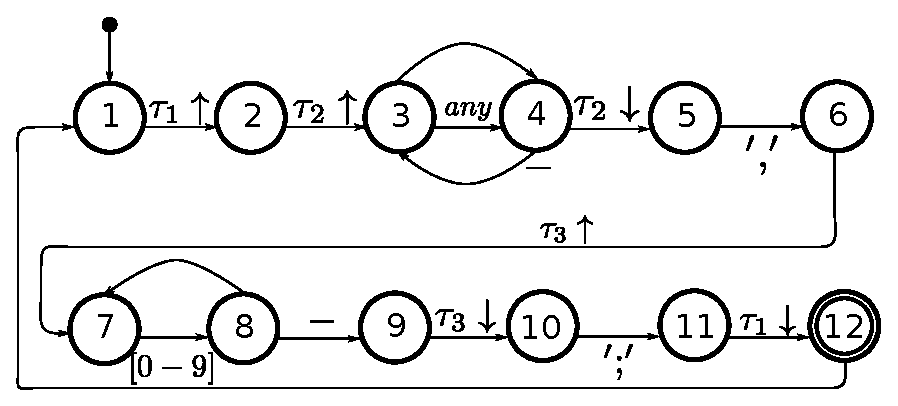
\includegraphics[width=\linewidth]{graphs/lehrer_automaton}

\caption[NFA for \texttt{((.*?),(\textbackslash{}d+);)+}]{\label{fig:example-automaton}
Automaton for \texttt{((.*?),(\textbackslash{}d+);)+}
In the diagram, ``$-$'' stands for low priority. $\tau_n\uparrow$ is the
opening tag for capture group $n$, likewise, $\tau_1\downarrow$ is the closing
tag for capture group $n$.}
\end{figure}

In the NFA, we model greedy repetition or non-greedy repetition of
an expression in two steps:

\begin{enumerate}
\item We construct an NFA graph for the expression, without any
repetition.  \autoref{fig:example-automaton} shows how this plays
out in our running example, which contains the expression \texttt{.*?}.
An automaton for expression~\texttt{.} is constructed. The expression
\texttt{.} is modeled as just two nodes labeled 3 and 4, and a
transition labeled ``any'' between them.

\item We add prioritized transitions to model repetition. In our
example, repeating is achieved by adding two $\varepsilon$ transitions:
one from 4 back to 3, to match more than one time any character,
and another one from 3 to 5, to enable matching nothing at all.
Importantly, the transition from 4 back to 3 is marked as low
priority (the ``--'' sign) while the transition leaving the automaton,
from 3 to 5, is unmarked, which means normal priority.  This means
that the NFA prefers leaving the repeating expression, rather
than staying in it.  If the expression were greedy, then we would
mark the transition from 3 to 5 as low-priority, and the NFA would
prefer to match any character repeatedly.

\end{enumerate}

More generally, the NFA prefers to follow transitions of normal
priority over those of low priority\footnote{See \Secref{tfsm}}.

\begin{figure*}[tb] 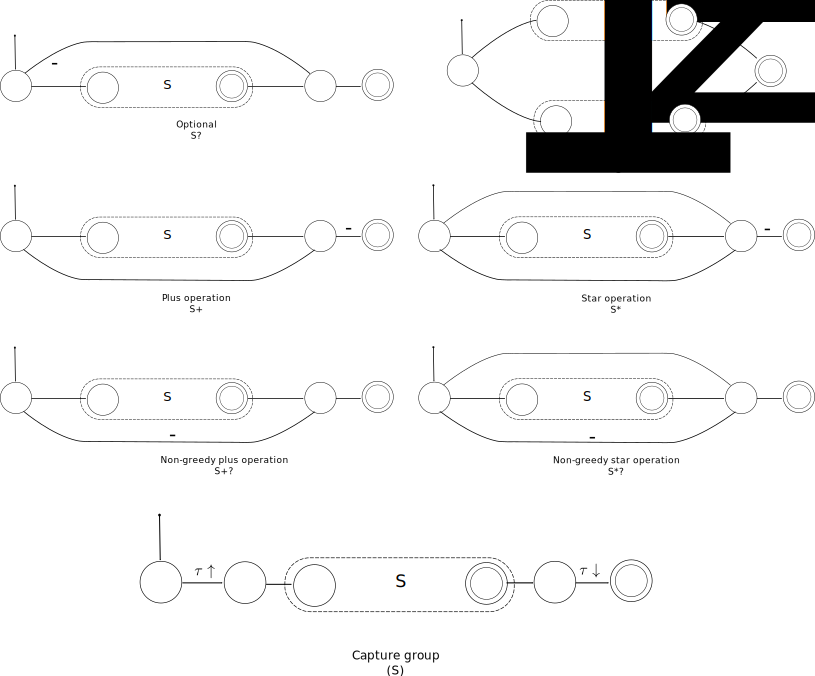
\includegraphics[width=\linewidth]{graphs/thompson}
  \caption[Modified Thompson construction]{Modified Thompson~\cite{Thom68a} construction of the
automaton: Descend into the abstract syntax tree of the regular
expression and expand the constructs recursively.}
\label{fig:thompson-construction}
\end{figure*}

\section{TNFA}	\seclabel{tnfa}

Our algorithm is directly based on algorithm~\ref{alg-coroutine-tagged}, so 
this section lays out the storage required by the co-routines and the
interpretation of the tags that we introduced in the previous section.

To model capture groups in the NFA, we add \emph{commit tags} to
the transition graph. The transition into a capture group is tagged
by a commit, the transition to leave a capture group is tagged by
another commit. We distinguish opening and closing commits. The
NFA keeps track of all times that a transition with an attached
commit was used, thus keeping the \emph{history} of each commit.
After parsing succeeds, the list of all histories can then be used
to reconstruct all matches of all capture groups.

\begin{figure}[htpb]
  \centering
  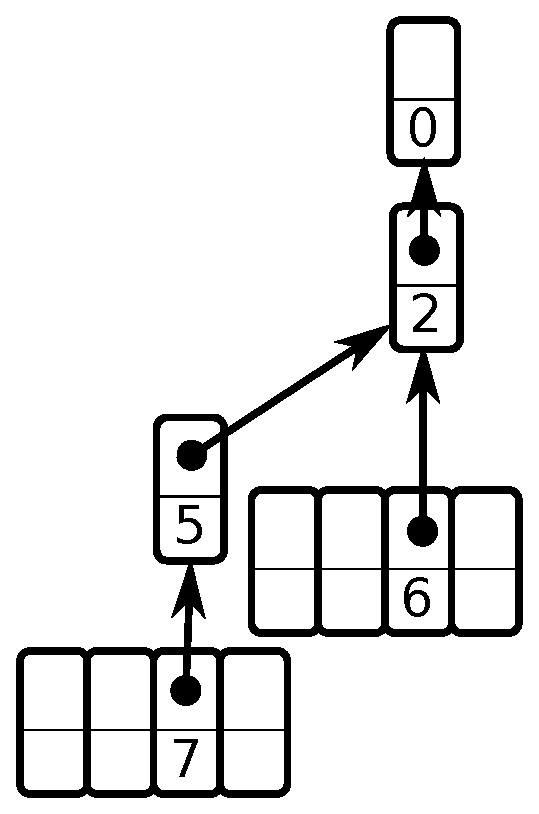
\includegraphics[height=7cm]{graphs/cells}
  \caption{Histories are cells of singly linked lists, where only the first 
    (here bottom-most) cell can be edited. This is a view of the automaton in 
    \Figref{example-automaton} after the string ``Tom Lehrer,1;Alan 
  Turing,'' has been consumed. Only the cell for the closing of the second 
capture group is shown.}
  \label{fig:cells}
\end{figure}

We model histories as singly linked lists, where the payload of each node is a
position.  Only the payload of the \emph{head}, the first node, is mutable, the
\emph{rest}, all other nodes, are immutable.  Because the rests are immutable,
they may be shared between histories.  This is an application of the flyweight
pattern, which ensures that all of the following instructions on histories can
be performed in constant time. Here, the \emph{position} is the current
position of the matcher.

\begin{notation}
We use the following vocabulary.

\begin{description}
\item[DFA states] are denoted by a capital letter, e.g. $Q$, and
	contain multiple co-routines.
  \begin{equation*}\begin{split}Q=[&(q_1, (h_1, h_2, h_3, h_4, h_5, h_6)),\\
	&(q_2, (h_1, h_2, h_3, h_4, h_7, h_8))]\end{split}\end{equation*} for example means
	that the current DFA state has one co-routine in NFA state $q_1$ with
	histories $(h_1, h_2, h_3, h_4, h_5, h_6)$ and another co-routine in NFA state
	$q_2$ with the histories $(h_1, h_2, h_3, h_4, h_7, h_8)$.
	Note that histories can be shared across co-routines if they
	have the same matches.
\item[Histories] are linked list, where each node stores a position in the
  input text.  The head is mutable, the rest is immutable. Therefore, histories
  can share any node except their heads. We write $h=[x_1, \dots, x_m]$ to
  describe that matches occurred at the positions $x_1, \dots, x_m$.
\item[Co-routines] are denoted as pairs $(q_i, h)$, where $q_i$ is some
	NFA state, and $h = (h_1, \dots, h_{2n})$ is an array of histories,
	where $n$ is the number of capture groups.  Each co-routine has an array
	of $2n$ histories. In an array of histories $(h_1, h_2, \dots
	h_{2n-1}, h_{2n})$, history $h_1$ is the history of the openings
	of the first capture group, $h2$ is the history of the closings of
	the first capture group, and so on.
\item[Transitions] are  understood to be between NFA states,
	$q_1\rightarrow q_2$ means a transition from $q_1$ to $q_2$.
\end{description}

Take for example the regular expression \texttt{(..)+} matching
pairs of characters, on the input string ``abcd''. The history array of the
finishing co-routine  is $[h_1=[0], h_2=[3], h_3=[2,0], h_4=[3,1]]$.
Histories $h_1$ and $h_2$ contain the positions of the entire match: position 0
through 3.  Histories $h_3$ and $h_4$ contain the positions of all the matches of
capture group 1, in reverse. That is: one match from 0 through 1, and another from
2 through 3.

Our engine executes instructions at the end of every interpretation
step. There are four kinds of instructions:

\begin{description}
\item [$h\leftarrow\pos$] Stores the current position into the head of history $h$.
\item [$h\leftarrow\pos+1$] Stores the position after the current one into the
  head of history $h$.
\item [$h'\mapsto h$] Sets head.next of $h$ to be head.next of $h'$.
	This effectively copies the (immutable) rest of $h$ to be the rest of $h'$, also.
\item [$c\uparrow(h)$] Prepends history $h$ with a new node that becomes the
  new head.  This effectively \emph{commits} the old head, which is henceforth
  considered immutable. $c\uparrow(h)$ describes the opening position of the
  capture group and is therefore called the opening commit.
\item [$c\downarrow(h)$] This is the same as $c\uparrow(h)$ except that it
  denotes a closing commit marking the end of the capture group.  This
  distinction is necessary, because an opening commit stores the position
  \emph{after} the current character and the closing commit store the
  position \emph{at} the current character.
\end{description}
\end{notation}

With this, the algorithm is simply implementing the fitting $interpret$
function as seen in algorithm~\ref{alg:coroutine-tagged}.

\begin{algorithm*}[htbp]
\begin{algorithmic}[1]
  \Function{$interpret$}{$t$, $m$}
    \If{$t$ is the character $c$}
      \If{$m$ is not fed and can current character is consumable by $c$}
      \State become fed
      \Else
        \State die
      \EndIf
    \EndIf
    \If{$t$ is $\varepsilon$}
      \If{$m$ is not fed}
        \State die
      \EndIf
      \State add new state to \emph{buffer}
    \EndIf
    \If{$t$ is open tag of group $i$}
      \State create new history $h$ as a copy of $m.histories[i]$
      \State write $index+1$ to history $h$
      \State create new memory $m'$, where $m'.histories[i] = h$
    \EndIf
    \If{$t$ is close tag of group $i$}
      \State create new history $h$ as a copy of $m.histories[i+1]$
      \State write $index$ to history $h$
      \State create new memory $m'$, where $m'.histories[i+1] = h$
      \State commit $m'.histories[i]$ and $m'.histories[i+1]$
    \EndIf
  \EndFunction
\end{algorithmic}
\label{alg:interpret}
\end{algorithm*}

The states are given to the algorithm in the order visited, so that the
coroutine that got furthest is expanded first when the next character is
read. The \emph{buffer} variable is a detail that ensures this.

Note that the ordering of co-routines inside of DFA states is relevant.
In \Figref{example-automaton}, after reading only one comma as an
input, state 7 can be reached from two co-routines: either from the
co-routine in state 3, via 4, or from the co-routine in state 6. The two
co-routines are `racing' to capture state 7. Since in the starting
state, the co-routine of state 6 is listed first, he `wins the race'
for state 7, and `captures it'. Thus, the new co-routine of state 7 is
a fork of the co-routine of state 6, not 3. This matters, since 6 and
3 may disagree about their histories.

\begin{example} Execution of algorithm~\ref{alg:coroutine-tagged} with the
  interpret as above:

Consider the automaton in figure~\ref{fig:example-automaton} is in
the DFA state\footnote{This is the starting state, except for the omission of
co-routines that would die immediately after scheduling because there are no
consuming transitions attached to their NFA state.}
\begin{align*}
Q=[
	(q_6, H_2=(&h_1, h_2, h_7,  h_8, h_5, h_6)), \\
	(q_3, H_1=(&h_1, h_2, h_3,  h_4, h_5, h_6))]
	\end{align*}
This is the case after initialization or before any commas are read.

The algorithm uses a stack \emph{lookat} with the possibility to push a low
priority transition below all high priority transitions\footnote{This is
easily implemented using two stacks, \emph{high} and \emph{low}.}.

We pretend for clarity that instructions are executed directly
after they are encountered.  The actual algorithm collects them and
executes them after the \emph{run} call to allow further
optimizations and the storage of the instructions.

Further, in the scope of this algorithm, co-routines have one extra bit of
information attached to them: they can be hungry or fed. Hungry co-routines can
only follow transitions that consume characters, fed co-routines can only
follow $\varepsilon$ transitions.

This is the execution of \emph{run}($Q$):

\begin{enumerate}
\item Fill the stack with hungry co-routines of all states of $Q$.
  Now, $\mathit{lookat}=[(q_6, H_2), (q_3, H_1))]$, where the first element
  is the head of the stack.
\item Initialize \emph{buffer} as an empty stack.
  The \emph{buffer} stack exists because while following high priority
  transitions, states are discovered in an order that is reversed with respect
  to the order in which we would like to output them.
\item Initialize $R=[\ ]$, the DFA state under construction.
\item co-routine $(q_6,H_2)$ is popped from the stack. It is hungry.
\item We iterate all available transitions in the NFA transition graph, and
  find only $q_6\rightarrow q_7$, which can consume character ``,''.
\item $(q_7, H_2)$ is pushed to the stack as fed, and we continue the main loop.
\item $(q_7, H_2)$ is taken from the stack. It is fed.
\item $(q_7, H_2)$ is pushed on \emph{buffer}.
\item Since $(q_7, H_2)$ is fed, it follows $\varepsilon$ transitions.
\item The available transition $q_7\rightarrow q_8$ is evaluated:
  \begin{enumerate}
    \item 	This transition has an opening tag for capture group 3 on it, and so we'd like to change $h_5$,
      the relevant history (see definition of $Q$ above). However, since we're \emph{spawning} a new co-routine, we cannot change $h_5$ itself.
      Instead, we copy $h_5$, and change the copy.
    \item	A new history $h$ is created.
    \item 	$h_5 \mapsto h$. Note that this is constant time, no matter how many entries $h_5$ already has.
    \item 	$h\leftarrow\pos+1$. This is the position after the ``,'', because the comma was eaten before the capture
        group starts.
    \item	Create $H_3 = [h_1, h_2, h_7, h_8, h, h_6]$ as a copy of $H_2$, with $h$ in the appropriate position.
    \item $(q_8, H_3)$ is pushed on the stack.
  \end{enumerate}
\item $(q_8, H_3)$ is taken from the stack.
\item It is pushed on \emph{buffer}. \emph{buffer}$=[(q_8, H_3), (q_7, H_2)]$
\item It can follow no further transitions and dies.
\item $(q_3, H_1)$ is popped from \emph{low}. It is hungry.
\item We now flush \emph{buffer}:
  $R=[(q_8, H_3), (q_7, H_2)]$, \emph{buffer}$=[\ ]$.  Note that now, $R$
  contains two co-routines in the reverse order in which they were discovered.
\item  $(q_3, H_1)$ is one of the two co-routines that constitute the
	input of this algorithm. Note how the other, $(q_6, H_2)$, got a
	chance to follow all of its transitions before $(q_3, H_1)$ was
	first popped off the low stack.
\item The only transition that consumes ``,'' is $q_3\rightarrow q_4$:\begin{enumerate}
	\item $(q_4, H_1)$ is pushed to the stack as a fed co-routine.
\end{enumerate}
\item $(q_4, H_1)$ is popped from the stack
\item It is pushed to the \emph{buffer}. \emph{buffer}$=(q_4, H_1)$
\item $q_4\rightarrow q_3$ is visited.
\begin{enumerate}
	\item co-routine $(q_3, H_1)$ is pushed to the stack after all high
    priority transitions (but there are none),
    because $q_4\rightarrow q_3$ has low priority.
\end{enumerate}
\item We flush the \emph{buffer} again: $R=[(q_8, H_3), (q_7, H_2), (q_4, H_1)]$
	Note how $(q_4, H_1)$ appears \emph{last} in $R$.
\item $(q_3, H_1)$ is taken from the stack.
\item It is added to \emph{buffer}.
\item $q_3\rightarrow q_5$ is visited:\begin{enumerate}
	\item $(q_5, H_1)$ is pushed to the stack.
\end{enumerate}
\item $(q_5, H_1)$ is taken from the stack.
\item It is added to \emph{buffer}.
\item $q_5\rightarrow q_6$ is visited and contains the closing commit of the
  second capture group:\begin{enumerate}
  \item Two histories are created to store the new positions of both the start
    and the end of the capture group. This ensures that other co-routines will
    not corrupt the memory.
	\item A new history $h$ is for the opening of the capture group.
	\item A new history $h'$ is created for the closing position.
  \item $h_3 \mapsto h$. See the definition of $Q$ above, to see that $h_3$ is
    the opening capture group position of $H_1$.
	\item $h_4 \mapsto h'$.
	\item $h'\leftarrow\pos$. This is the position of the ``,''.
	\item Create a new history array, with $h$ and $h'$ in place.
		$H_4 = [h_1, h_2, h, h', h_5, h_6]$
	\item $(q_6, H_4)$ is pushed to the stack.
\end{enumerate}
\item $(q_6, H_4)$ is taken from the stack.
\item It is added to the \emph{buffer}.
\item The stack is empty.
\item We flush our \emph{buffer}:
\begin{align*}
R=[&(q_8, H_3), (q_7, H_2), (q_4, H_1),\\ &(q_6, H_4), (q_5, H_1), (q_3, H_1)]
\end{align*}
\item $R$ is returned.
\end{enumerate}
\end{example}

The output contains six co-routines, but three of them,  $(q_7, H_2)$,
$(q_4, H_1)$,  $(q_5, H_1)$, will die as soon as they are scheduled in
the next iteration of the algorithm, because there are no outgoing
non-$\varepsilon$ transitions attached to their NFA states.

The overall run time of algorithm \ref{alg:coroutine-tagged} depends heavily on the
forking of co-routines being efficient: In the worst case, it takes
$\Theta(m\, T_{fork}(m))$ time. A naive solution is a copy-on-write array, for
which $T_{fork}(m)=m$ gives $O(m^2)$ for every character read, resulting
in $O(n\,m^2)$ regular expression matching, which is only acceptable
if we assume $m$ to be fixed.

Since at most two histories are actually changed, much of the
array would not be modified and could be shared across the original
co-routine and the forked one. This is easily achieved replacing the
array by a persistent~\cite{Dris89a} data structure to hold the
array. A persistent treap, sorted by array index, has all necessary
properties\footnote{Clojure~\cite{Hick08} features a slightly more complex data
structure under the name of `persistent vectors'. Jean Niklas L'orange offers a
good explanation in ``Understanding Clojure's Persistent Vectors'',
\url{http://hypirion.com/musings/understanding-persistent-vector-pt-1}.} and
is further elaborated upon in \Secref{treap}. With $T_{fork}=O(\log m)$,
the overall runtime is $O(n\,m\,\log m)$.

\chapter{Data structures}\label{cha:data}
In the previous chapter, we obtained an algorithm with a run-time
proportional to the cost of storing updates in a fixed size data structure
with one access and one update. This needs to be fully
persistent\footnote{This means that old versions of the data structure are
  still accessible and can be forked so that a new data structure with only
that change applied can be accessed.} in order to allow for co-routine forking.

This chapter presents some possible data structures, that allow for this.

\section{Fully persistent data structures}	\seclabel{treap}\seclabel{data-structures}
In order to allow modifications of our list of histories, it is
necessary to build a data structure that provides the interface a guarantees
of a copy-on-write array:

\begin{definition}
  An \texttt{Arraylike} data structure $A$ of length $m$ must provide the
  following interface:
  \begin{description}
    \item[Constructor] $A(m)$ must return a structure of length $m$.
    \item[Random access] An instance of $A$ must provide a method $get(i)$,
      which gives a history for each $0 \leq i < m$.
    \item[Setting elements] An instance of $A$ must provide a method $set(i,
      history)$, which returns a new version of $A$, so that $get(i) = history$.
      The original instance must still return the same value for any $get$
      and $set$ -- it must be logically unmodified.
  \end{description}

  This is a definition of a fixed-size fully-persistent linear data structure.
\end{definition}

Note that multiple versions of the data structure can change, every version
that is in a living co-routine. A way to visualize this is as a tree of
versions, where each $set$ call forks off a new node, as seen in
\Figref{version-tree}.

\begin{figure}[htpb]
  \centering
  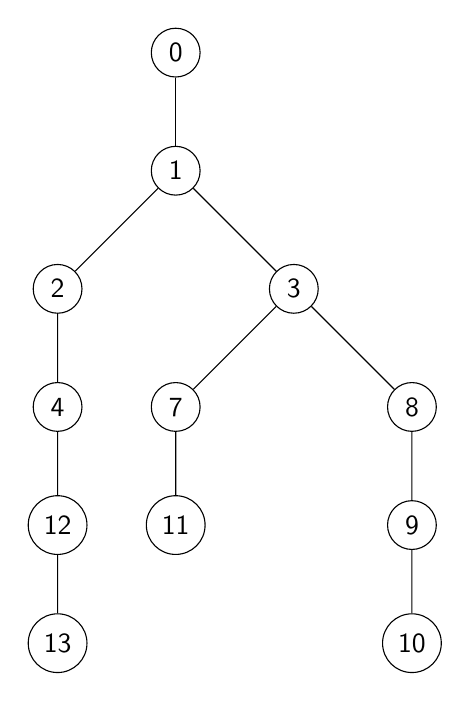
\begin{tikzpicture}[
every node/.style = {align=center, text centered,
font=\sffamily, circle, draw=black}, level/.style={
sibling distance=3cm} ]
\node {0}
child {
  node {1}
  child {
    node {2}
    child {
      node {4}
      child {
        node {12}
        child {
          node {13}
        }
      }
    }
  }
  child {
    node {3}
    child {
      node {7}
      child {
        node {11}
      }
    }
    child {
      node {8}
      child {
        node {9}
        child {
          node {10}
        }
      }
    }
  }
};
  \end{tikzpicture}
  \caption{A tree of versions. Forks in the tree mean that multiple threads
  forked from the same state in the TNFA. The labels describe be the relative
order of creation. It isn't linear.}
  \figlabel{version-tree}
\end{figure}

The rest of this section looks at different possible implementations and
their relative performance. Since in the worst case $get$ as well as $set$ are
required in each step of each co-routine, the relevant performance measure is
$T=O(T_{get} + T_{set}) = O(max(T_{get}, T_{set}))$ measured in amortized time.

\section{Copy-on-write array}
The arguably simplest class to provide the interface is an array that copies
itself before making modifications:

\begin{description}
  \item[Constructor] $A(m)$ allocate an array of histories $a$ of size $m$.
  \item[Random access] $get(i)$ gives the $i$th element of the array in $O(1)$
    time.
  \item[Setting elements] $set(i, history)$ copies $a$ and set the $i$th
    element to be $history$. This takes $O(m)$ time.
\end{description}

The performance for $get$ and $set$ gives us $T=O(1 + m) = O(m)$.

While the asymptotic performance is abysmal, the copy-on-write array is not
to be dismissed apriori, since it has great memory locality properties and
might outperform more complex structures for small $m$.

\section{Treap}
The treap data structure allows copy-on-write in $\log m$ time, sharing
much of the structure by using the flyweight pattern as can be seen in
\Figref{treap}. The treap is a balanced, left-leaning binary tree with entries
in each node, equipped with the operations \texttt{get} and \texttt{set} as follows.

\begin{algorithm*}
\begin{algorithmic}[1]
\Function{get}{treap, index}
	\If{$\text{index} = 0$}
		\State \Return treap.entry
	\ElsIf{$\text{index}-1 < \text{treap.left.size}$}
		\State \Return \Call{get}{treap.left, $\text{index}-1$}
	\Else
		\State \Return \Call{get}{treap.right, $\text{index}-\text{treap.left.size}-1$}
	\EndIf
\EndFunction
\Statex
\Function{set}{treap, index, entry}
	\If{$\text{index} = 0$}
		\State $\text{treap}'\gets copy(treap)$
		\State $\text{treap}'\text{.entry} \gets \text{entry}$
		\State \Return treap'
	\ElsIf{$\text{index}-1 < \text{treap.left.size}$}
		\State $\text{treap}'\gets copy(\text{treap})$
		\State $\text{treap}'\text{.left} \gets \Call{set}{\text{treap.left}, \text{index}-1, \text{entry}}$
		\State \Return $\text{treap}'$
	\Else
		\State $\text{treap}'\gets copy(\text{treap})$
		\State $\text{treap}'\text{.left} \gets \Call{set}{\text{treap.right}, \text{index}-\text{treap.left.size}-1, \text{entry}}$
		\State \Return $treap'$
	\EndIf
\EndFunction
\end{algorithmic}
\caption{\label{alg:treap} Implementation of the treap methods}
\end{algorithm*}

\begin{figure}
\resizebox{\linewidth}{!}{
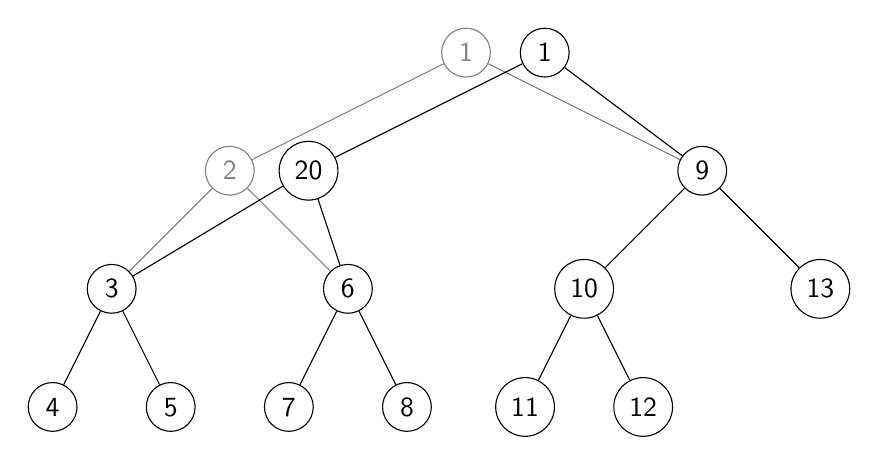
\begin{tikzpicture}[>=stealth',level/.style={
level 1/.style={sibling distance=6cm},
level 2/.style={sibling distance=3cm},
level 3/.style={sibling distance=1.5cm}},
every node/.style = {align=center, text centered,
    font=\sffamily, circle, draw=black},
norm/.style={edge from parent/.style={black,thin,draw}},
hiddentree/.style={edge from parent/.style={gray,thin,draw}}]
\node [gray, hiddentree] (n1) {1}
	child [hiddentree] {
		node [gray] (n2) {2}
			child [hiddentree] {
				node (n3) {3}
				child [norm] { node {4} }
				child [norm] { node {5} }
			}
			child [hiddentree] {
				node (n6) {6}
				child [norm] { node {7} }
				child [norm] { node {8} }
			}
		}
	child [hiddentree] {
		node (n9) {9}
			child [norm] {
				node{10}
				child {	node{11} }
				child { node {12} }
			}
			child [norm] {node {13} }
		} ;

\node (n1p) [right of=n1] {1};
\node (n2p) [right of=n2] {20};
\path (n1p) edge (n2p);
\path (n2p) edge (n3);
\path (n2p) edge (n6);
\path (n1p) edge (n9);
\end{tikzpicture}}
\caption[Treap for history storage]{\figlabel{treap}Writing to the second entry of the treap only requires
$O(\log m)$ copies while keeping the old structure intact (persistence).}
\end{figure}

This structure gives us better asymptotic performance at the cost of
following $\log m$ pointers, because $T = O(\log m + \log m) = O(\log m)$.

\section{Storing updates}
Driscoll et al\cite{Dris89a} describe how any pointer machine data structure
with a fixed number of links to each version can be converted to a fully
persistent data structure in $O(1)$ amortized time. This section shows
the steps involved to equip an array with such an interface.

The idea behind the conversion is that instead of modifying the array
directly, we instead keep a buffer of modifications that is of fixed
size. Let's for the moment assume that we have a linear order of modifications
and only add the version tree later.

\subsection{Linear versions}
In this part, we only modify the most recent version $t^\star$ and only
access the old versions $0 \leq t \leq t^\star$. In order to store the
modifications, we introduce the struct $Set(t, i, history)$, which can be stored
in the modification buffer. The implementation of the simple methods can be
seen in algorithm~\ref{alg:lazy-apply-1}

\begin{algorithm*}
\begin{algorithmic}[1]
\Function{makeLazyApply}{m}
  \State allocate an array of $m$ histories $hs$
  \State allocate a buffer $b$ of size $p$ for modifications.
  \State \Return $\{ histories: hs, buffer: b\}$
\EndFunction
\Function{get}{lazyApply, t, index}
  \State $history \leftarrow lazyApply.histories[index]$
  \For{each $Set(t', i, history')$}
    \If{$t' < t$ and $i = index$}
      \State $history \leftarrow history'$
    \EndIf
  \EndFor
  \State \Return $history$
\EndFunction
\Statex
\Function{set}{lazyApply, t, index, entry}
  \If{$lazyApply.buffer$ has space left}
    \State add $Set(t, index, entry)$ to $lazyApply.buffer$
    \State \Return $lazyApply$
  \Else
    \State\Return new $LazyApply$ with all changes applied
  \EndIf
\EndFunction
\end{algorithmic}
\caption{\label{alg:lazy-apply-1}Methods of the $LazyApply$ data structure}
\end{algorithm*}

The amorized constant time for $get$ and $set$ arise from the fact that while
we iterate through the changes, we only have a constant number of them.

\subsection{Version tree}
In the general case of a version tree, we lose the notion of a total order of
versions and remain with a partial order. Version $t_1$ and version $t_2$ can
now be in three different relations: Either $t_1$ can happen before $t_2$, so
that the modification in $t_1$ also needs to be taken into account in $t_2$,
$t_2$ can happen before $t_1$, or they can be siblings, so that the
modifications shouldn't influence each other.

The problem of generalizing this approach to version trees is two fold: The
first problem is, that we need to determine whether a modification applies to a
version in constant time, otherwise $get$ would become slower. The second
problem is that modifying the same version reduces to copying the array of
histories if said version has a full buffer. The latter is more easily solved
and thus will be discussed first.

\paragraph{Emptying a full buffer} Instead of applying all modifications, we
can split the modification buffer in two roughly equal parts. In order to do
that, we can find a subtree $v$ of modifications of size $\approx \frac{p}{2}$.
Instead of applying all modifications to the array of histories, we only
apply the ancestors of $v$. Then we delete all modifications in $v$ from the
original node. Now we would be breaking the interface, because some
co-routines still have references to the original node, but actually use a
version that is in $v$. This can be avoided by storing back-pointers to the
threads and modify their references to the new node if necessary. Since there
are at most $m$ threads referencing the versions of each node, we can still
update the references in amortized constant time.

\paragraph{Constant time ordering of versions}
In order to determine whether to apply a modification on a read, we need to
find the relation between the version that is querried and the one that is
stored. If $t_{stored} < t_{querried}$, we apply the modification. This
requires us however to determine the relative positions of $t_{stored}$ and
$t_{querried}$ in the version tree, where the naive implementation would take
$\log m$ time. This is the order maintenance problem and fittingly can be
solved using an order maintenance data structure, such as the one proposed by
Dietz and Sleator\cite{Diet87b} which we discuss in \Secref{order-maintenance}.

For the moment let us assume that we have a linear data structure, that
\begin{enumerate}
  \item allows inserting an element next to a known element in $O(1)$ time.
  \item allows us to query the order of two elements $a$ and $b$ in the list
    in $O(1)$ time. We'll call this operation $query_<(a, b)$.
\end{enumerate}

With this we can flatten the tree to a list by adding a $b_t$ beginning
element and an $e_t$ closing element to the list as seen in
\Figref{flattening-tree}.

\begin{figure}[htpb]
\resizebox{\linewidth}{!}{
\begin{tikzpicture}[>=stealth',level/.style={
level 1/.style={sibling distance=5cm},
level 2/.style={sibling distance=2.5cm}},
every node/.style = {align=center, text centered,
    font=\sffamily, circle, draw=black}]
\node (n1) {$v_1$}
	child {
		node (n2) {$v_2$}
    child { node (n3) {$v_3$} }
    child { node {$v_4$} }
  }
  child { node (n5) {$v_5$} } ;
\node (o3) [below=0.0cm of n3, draw=none,fill=none] {$(b_1\ (b_2\ (b_3\ e_3)$};
\node (o4) [draw=none,fill=none, right=0.5cm of o3] {$(b_4\ e_4)\ e_2)$};
\node (o5) [draw=none,fill=none, right=of o4] {$(b_3\ b_3)\ e_1)$};
\end{tikzpicture}
}
  \caption{A flattened version tree}
  \label{fig:flattening-tree}
\end{figure}

Now we can find if version $t_2$ depends on version $t_1$, by calculating
\[ query_<(b_{t_1}, b_{t_2})\ \mathrm{\&\&}\ query_<(e_{t_2}, e_{t_1})\]
If $t_1$ encloses $t_2$ completely, then $t_2$ is part of the subtree of $t_1$
and therefore we'd need to apply the modification at $t_1$ to find values at
$t_2$.

\section{Order maintenance}\seclabel{order-maintenance}
Dietz and Sleator describe in their paper Two Algorithms for Maintaining
Order in a List\cite{Diet87b}\footnote{And Bender et al\cite{Bend02a} in
their revision of this classical paper}, a simple one that provides amortized
guarantees and a more involved one, which could offer worst-case guarantees.
For our purposes the amortized version suffices, as noted by Driscoll et
al\cite[p. 108]{Dris89a}.

The data structure keeps so called \emph{tags} $\eta(e)$ for elements, which are
integers that describe the order. In order to query the relative position of
two elements, their tags are simply compared, which leaves us with the
problem of maintaining tags for all list elements such that
$\eta(e_1)<\eta(e_2) \Leftarrow index(e_1) < index(e_2)$.

Compare this to the related problem of list-labeling: in order maintenance we
need to be able to compute the full label for each element in constant time,
whereas in list-labeling, the node has to contain the full label itself. This
insight is key to maintaining order in amortized constant time. For the moment
however we look at the method we can use for list-labeling.

The key to achieve this is to use a doubly linked list of tags with their
corresponding elements. If we need to insert an element after another known
element $e$, we can insert it, but to keep our invariant, we assign
$\eta(e_{new}) =\floor*{\frac{\eta(e) + \eta(e.next)}{2}}$. This is possible,
unless the new tag is actually equal to $\eta(e)$ -- if $\eta(e)$ doesn't
have any space to $\eta(e.next)$. In this case we need to relabel the
existing nodes.

\subsection{Relabeling}
The purpose of the relabeling step is to ensure that there is a gap to fit
in the new element and reduce the potential of a next reordering step. An
intuitive perspective is shown by Bender et al\cite{Bend02a}:

The labels can be thought of a coding of paths in a complete binary tree as
visualized in \Figref{labels-bin-tree}. We can then define the
\emph{overflow} in a subtree, which triggers relabeling.

\begin{figure}[htb]
  \centering
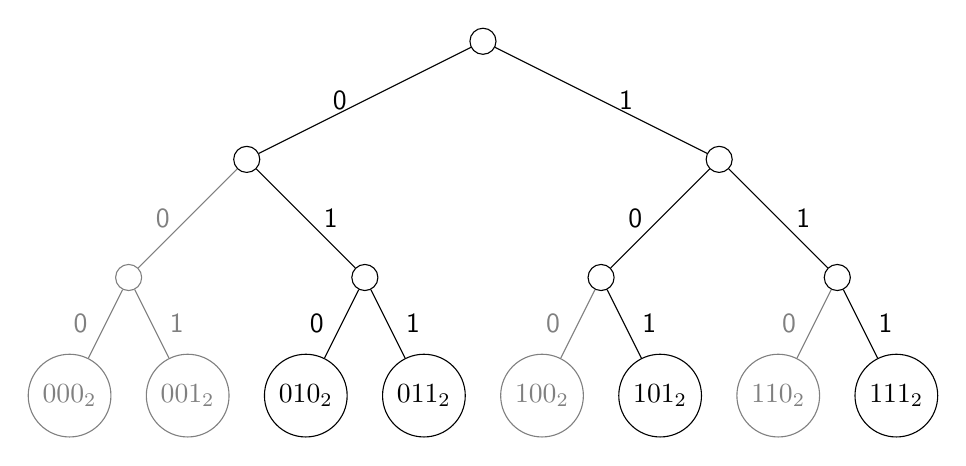
\begin{tikzpicture}[>=stealth',level/.style={
level 1/.style={sibling distance=6cm},
level 2/.style={sibling distance=3cm},
level 3/.style={sibling distance=1.5cm}},
every node/.style = {align=center, text centered,
    font=\sffamily, circle, draw=black},
norm/.style={edge from parent/.style={black,thin,draw}},
hiddentree/.style={edge from parent/.style={gray,thin,draw}}]
\node {}
  child {
    node {}
    child [hiddentree] {
        node [gray] {}
        child { node [gray] {$000_2$}  edge from parent node[left,draw=none] {0} }
        child { node [gray] {$001_2$}  edge from parent node[right,draw=none] {1} }
        edge from parent node[left,draw=none] {0}
			}
			child {
        node {}
        child {node {$010_2$} edge from parent node[left,draw=none] {0} }
        child {node (n6) {$011_2$} edge from parent node[right,draw=none] {1} }
        edge from parent node[right,draw=none] {1}
			} edge from parent node[left,draw=none] {0}
		}
	child {
		node {}
			child {
        node {}
        child [hiddentree] { node [gray] {$100_2$}  edge from parent node[left,draw=none] {0} }
        child { node {$101_2$}  edge from parent node[right,draw=none] {1} }
        edge from parent node[left,draw=none] {0}
			}
			child {
        node {}
        child [hiddentree] {node [gray] {$110_2$} edge from parent node[left,draw=none] {0} }
        child {node {$111_2$} edge from parent node[right,draw=none] {1} }
        edge from parent node[right,draw=none] {1}
			} edge from parent node[right,draw=none] {1}
		} ;
\end{tikzpicture}
\caption[Tree for relabeling order]{Labels are binary numbers describing paths in a tree. Relabeling
  walks up the tree until it finds a subtree with a density below the
threshold. In this range, the labels changed to make them equally spaced.}
  \label{fig:labels-bin-tree}
\end{figure}

\begin{defn}
  The \emph{overflow threshold} of a subtree is $1.5^i$ for any
  level\footnote{$a=1.5$ is an arbitrary choice for a number $1 < a < 2$.} $i$,
  starting counting from the leafs, which are level 0.

  \emph{Overflow} happens, when the number of items in a subtree are bigger
  than the overflow threshold.
\end{defn}

With this definition, we can define the region that we relabel to be the
first subtree that isn't in overflow -- which means that is is filled
sufficiently sparsely to reduce the potential new relabels. In this subtree
we spread the labels equally, which ensures that we will not have to
do any relabeling for another $\floor{1.5^{-i}}$ inserts. Note that a much
bigger region might be in overflow, but no checks are done if they are not
triggered by an overflow at level 0, i.e.\ placing a node between two adjacent
nodes.

This algorithm leaves us with the disappointment of only achieving $O(\log m)$
amortized insert. This can be resolved using a technique known as
\emph{indirection}.

\subsection{Indirection}
Indirection is a method introduced by Willard\cite{Will82a} to eliminate
annoying $\log$ factors under certain conditions such as the one just
encountered.  With it we leave the realm of list-labeling and cease to store
the full label in each node. Instead we now keep a two-level structure
as shown in \Figref{graphs/indirection}.

\begin{figure}[htpb]
  \centering
  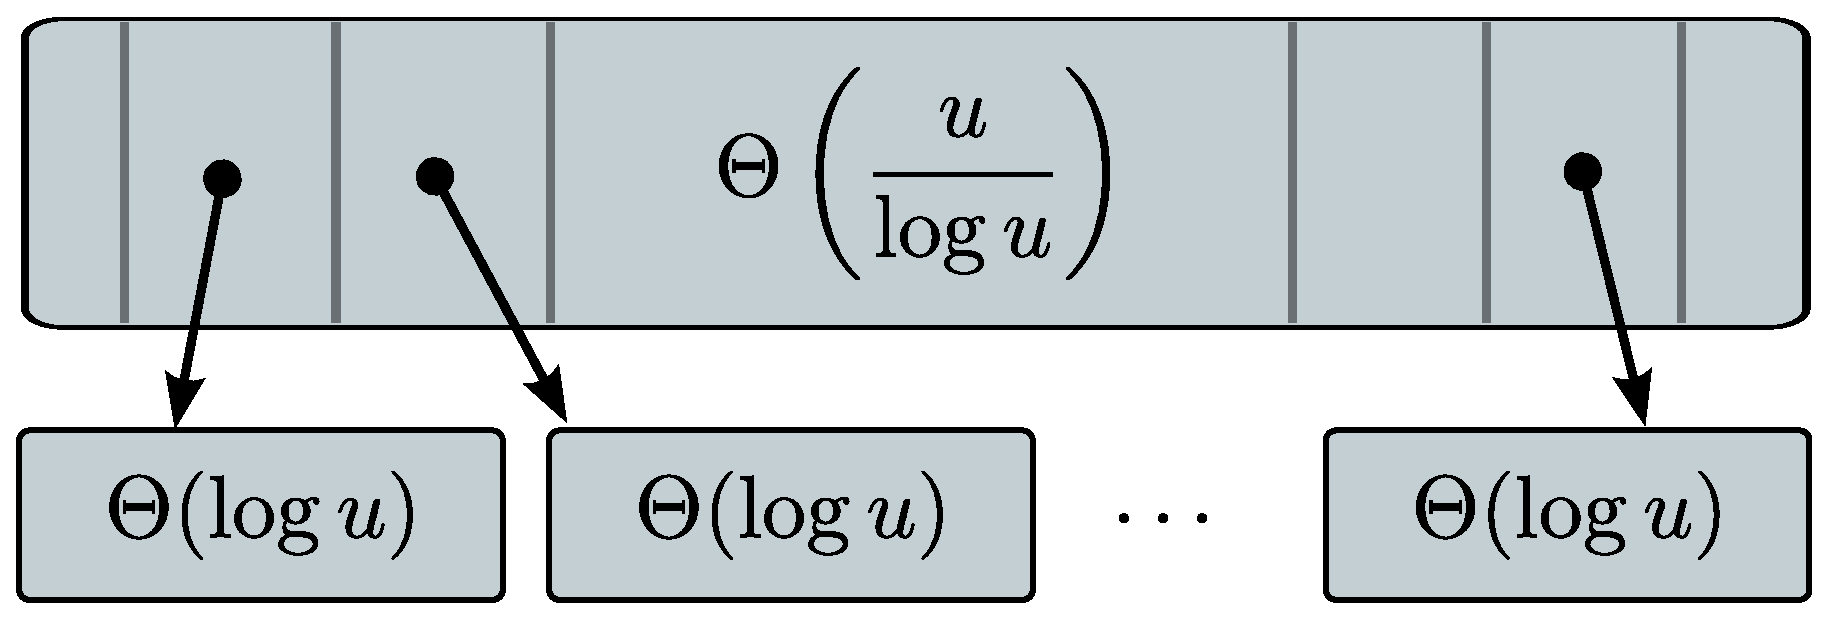
\includegraphics[width=0.8\linewidth]{graphs/indirection}
  \caption{Indirection structure: use a compound index with the high-order
  bits being the index for the upper structure and the low-order bits being
the index for the lower structure. Since the upper index is stored in the
summary structure, $\log u$ items can be relabeled in $O(1)$ time.}
  \figlabel{graphs/indirection}
\end{figure}

We split our universe into blocks of size $\Theta(\log u)$. In these blocks we keep a
labeled list as seen in the previous section. Above this, we create a summary
structure, which stores a second part of the index. This too is a labeled
list, but since each element of the summary structure represents
$\Theta(\log u)$ elements of the universe, we can effectively do relabels
faster by a $\log$-factor. This gives us amortized $O(1)$ updates.

It can be said that this seems to set a limit on the size of the match: Once
our labels are used up, we cannot do $O(1)$ order queries anymore. This is
true, but there is a smaller limit already in place: We can't store pointers
to a string that doesn't fit into memory. If we cease to understand positions
as fixed in size, we would again get a $\log$-factor. This is typically not
considered.

\chapter{Proofs}
In this chapter we will prove the claimed properties, first and foremost the
correctness of the algorithm.

\section{Correctness}
The correctness of the algorithm follows by induction over the construction:
If the correct co-routine stops in the end state for all possible
constructions of the Thompson construction under the assumption that simpler
automata do the same, it follows that no matter how complex the automata get,
the algorithm will have the correct output.

To this goal, we will use backtracking as a handy definition of correctness.
We will show that our algorithm will prefer the same paths as a backtracking
implementation would. It should be noted that the construction is exactly
set up so that it matches backtracking and in fact this can be seen as a
simple derivation of our algorithm.

First we need a simple formalization of the backtracking procedure:

\begin{align*}
  bt(a|b, s) &= bt(a, s)\qquad | \qquad bt(b, s)\\
  bt(r*, s) &= bt(rr*|\varepsilon, s)\\
  bt(r*?, s) &= bt(\varepsilon|rr*, s)\\
  bt(r?, s) &= bt(r|\varepsilon, s)\\
  bt(r??, s) &=  bt(\varepsilon|r, s)\\
  bt(r+, s) &= bt(rr*, s)\\
  bt(r+?, s) &= bt(rr*?, s)\\
  bt(ab, s) &= bt(a, s) + bt(b, rest)\\
  bt(Group(i, r), s) &= [WriteOpen(i)] + bt(r, s) + [WriteClose(i)]
\end{align*}

Second we notice that the algorithm preserves the order of the co-routines
after each character read. This means that basically a depth first search
is performed, with priorities formalizing what option is to be taken first.

That certain paths are cut off, because the state has already been seen is
equivalent to memoization in the backtracking procedure: If a higher priority
state already found a path through this part of the parse, the following
parse can be pruned.

Now the parses are analogous for our procedure and $bt$:

\begin{center}
  \begin{tabular}{p{5cm}|p{7cm}}
    \hline \hline
    $bt(a|b, s)$:\begin{enumerate}
      \item Check $a$
      \item Check $b$
    \end{enumerate}
    &  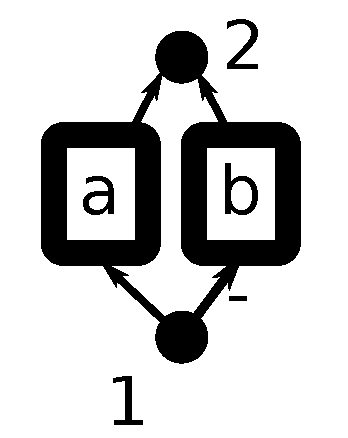
\includegraphics[width=3.5cm]{graphs/ror}
    \begin{enumerate}
      \item Check $1\rightarrow a\rightarrow 2$
      \item Check $1\rightarrow b\rightarrow 2$
      \end{enumerate} \\ \hline
    $bt(r*, s)$:\begin{enumerate}
      \item Check $r$
      \item Check $\varepsilon$
    \end{enumerate}
    & 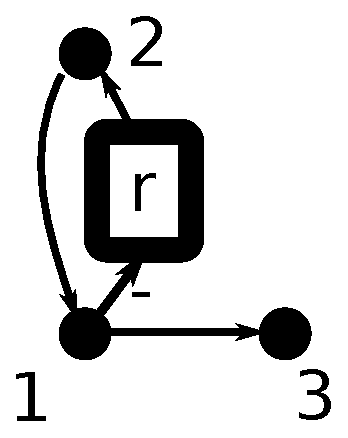
\includegraphics[width=3.5cm]{graphs/rstar}
    \begin{enumerate}
      \item Check $1\rightarrow r\rightarrow 2\rightarrow 1\rightarrow 3$
      \item Check $1\rightarrow 3$
      \end{enumerate}\\
      $$\vdots$$& $$\vdots$$\\
      \hline
  \end{tabular}
  \\
  \begin{tabular}{p{5cm}|p{7cm}}
    \hline
    $bt(ab, s)$: \begin{enumerate}
      \item Check $a$
      \item Check $b$ on rest
      \item Concatenate the updates
    \end{enumerate}
    & 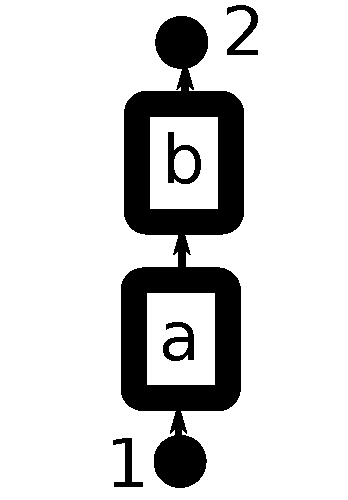
\includegraphics[width=3.5cm]{graphs/rseq}
    \begin{enumerate}
      \item Run through $a$ consuming some characters
      \item Run through $b$
      \item All changes are written
    \end{enumerate} \\
    \hline
    $bt(Group(i, r), s)$: \begin{enumerate}
      \item Write current position to changes
      \item Check $r$
      \item Write position after matching $r$ to changes
    \end{enumerate}
    & 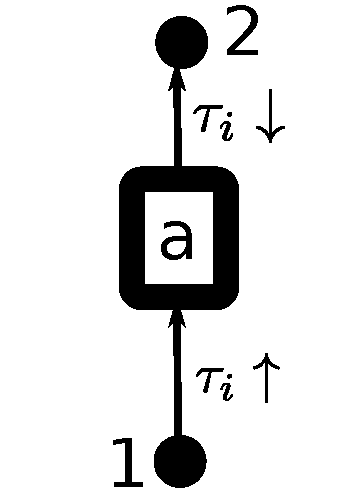
\includegraphics[width=3.5cm]{graphs/rgroup}
    \begin{enumerate}
      \item Write current position to changes
      \item Run through $r$
      \item Write the changed position to changes
    \end{enumerate} \\
    \hline \hline
  \end{tabular}
\end{center}

\section{Execution time}
The main structure of any NFA based matching algorithm is the nesting of two
loops: The outer loop iterating over the $n$ characters of the string, and
the inner expanding at most $m$ states. The expansion makes $O(1)$ updates
per state expanded, as the construction described in
section~\ref{sec:nfa-match} gives a constant out-degree for each state. As
described in chapter~\ref{cha:data} the update cost of every co-routine is
$O(1)$. This gives a total run time of $O(n\, m)$.

\section{Lower bound for time}\seclabel{lower-bound}
There is no known tight\footnote{A lower bound $l$ is tight, if it is the
asymptotically largest lower bound} lower bound to regular expression
matching.

\begin{thm}
  No algorithm can correctly match regular expressions faster than
  $\Theta(n\, \min(m, \abs{\Sigma}))$, where $n$ is the length of the string,
  $m$ is the length of the pattern, and $\abs{\Sigma}$ is the size of the alphabet.
\end{thm}
\begin{proof}
  Let $S=a^nx_i$ and $R=\mathtt{[ax_1]*|[ax_2]*|\dots|[ax_m]*}$. Note that
  $\abs{S} = \Theta{n}$ and $\abs{R}=\Theta(\min(m, \abs{\Sigma}))$. Let
  further \texttt{match} be a valid regular expression matching algorithm,
  then $\mathtt{match}(S, R)$ is equivalent to finding
  $a^nx_i\stackrel{?}{\in} \{a^nx_1, \dots, a^nx_m\}$. There is no particular order to
  $\{a^nx_1, \dots, a^nx_m\}$, so the lower bound for finding this is
  $\Theta(\abs{S}\, \abs{R})$.
\end{proof}

\chapter{Implementation}
While repeatedly calling algorithm \ref{alg:coroutine-tagged} would be sufficient
to reach the theoretical time bound we claimed, practical performance
can be dramatically improved by avoiding to construct new states.
Instead, we build a \emph{transition table} that maps from old DFA
states and an input range to a new DFA state, and the instructions
to execute when using the transition. We build the transition table,
including instructions, as we go. This is what we mean when we say
that the DFA is \emph{lazily compiled}.

\section{DFA transition table}
The DFA transition table is different from the NFA transition table,
in that the NFA transition table contains $\varepsilon$ transitions and
may have more than one transition from one state to another, for
the same input range. DFA transition tables allow no ambiguity.

Our transition tables, both for NFAs and DFAs, assume a transition
to map a consecutive range of characters. If, instead, we used
individual characters, the table size would quickly become unwieldy.
However, input ranges can quickly become confusing if they are
allowed to intersect. To avoid this, and simplify the code dramatically,
while keeping the transition table small, we use the following
trick. When the regular expression is parsed, we keep track of all
input ranges that occur in it. Then, we split them until no two
input ranges intersect.  After this step, input ranges are never
created again.  Doing this step early in the pipeline yields the
following invariant: it is impossible to ever come across intersecting
input ranges.

To give us a chance to ever be in a state that is already in the
transition table, we check, after executing algorithm~\ref{alg:coroutine-tagged},
\texttt{run}, whether there is a known DFA state that is
\emph{mappable} to the output of \texttt{run}.  If \texttt{run}
produced a DFA state $Q$, and there is a DFA state $Q'$ that contains
the same NFA states, in the same order then $Q$ and $Q'$ may be
mappable.  If they are, then there is a set of instructions that
move the histories from $Q$ into $Q'$ such that, afterwards, $Q'$
behaves precisely as $Q$ would have. Algorithm~\ref{findmapping}
shows how we can find a mappable state, and the needed instructions.
The run time of Algorithm~\ref{findmapping} is $O(m)$, where $m$
is the size of the input NFA.

\begin{algorithm*}[htpb]
\begin{algorithmic}[1]
\Require{$Q=[(q_i, h_i)]_{i=1\dots n}$ is a DFA state.}
\Ensure{A state $Q'$ that $Q$ is \emph{mappable} to.\\
	The ordered instructions $m$ that reorder the memory
		locations of $Q$ to $Q'$ and don't interfere with each other.}

\For{$Q'$ that contains the same NFA states as $Q$, in the same order}

	\LineComment{Invariant: For each history $H$ there is at most one $H'$\\ so that $H\leftarrow H'$ is part of the mapping.}
	\State Initialize empty bimap $m$ \Comment{A bimap is a bijective map.}

	\For{$q_i=q'_i$ with histories $H$ and $H'$ respectively}
		\For{$i=0\dots length(H)-1$}


			\If{$H(i)$ is in $m$ as a key already and does not map to $H'(i)$}
				\State Fail
			\Else
				 \LineComment{Hypothesize that this is part of a valid map}
				\State Add $H(i) \mapsto H'(i)$ to $m$
			\EndIf
		\EndFor
    \EndFor
\EndFor
\LineComment{The mapping was found and is in $m$.}

	\State sort $m$ in reverse topological order so that no values are overwritten.

	\Return{$Q'$ and $m$}
  \caption[$findMapping(Q)$]{\label{findmapping}$findMapping(Q)$: Finding a state that $Q$ is
mappable to in order to keep the number of states created bound by the length
of the regular expression.}
\end{algorithmic}
\end{algorithm*}

\section{DFA execution}
With these ingredients in place, the entire matching algorithm is
straightforward.  In a nutshell, we see if the current input appears
in the transition table. Otherwise, we run \texttt{run}. If the
resulting state is mappable, we map.  More formally, we can see
this in algorithm~\ref{interpret}. Here, algorithm~\ref{interpret}
assumes that algorithm~\ref{alg:coroutine-tagged} does not immediately execute
its instructions, but returns them back to the interpreter, both for
execution and to feed into the transition table.

\begin{algorithm*}[htpb]
\begin{algorithmic}[1]
\Require{$input$ is a sequence of characters.}
\Ensure{A tree of matching capture groups.}
\LineComment{Lazily compiles a DFA while matching.}

\State Set $Q$ to \emph{startState}.
\LineComment{A co-routine is an NFA state, with an array of histories.}
\State Let $Q$ be all co-routines that are reachable in the NFA transition graph by following $\varepsilon$ transitions only.
\State Execute instructions described in algorithm \emph{run}, when walking $\varepsilon$ transitions.

\LineComment{Create the transition map of the DFA.}
\State Set $T$ to an empty map from state and input to new state and instructions.
\LineComment{Consume string}
\For{position $pos$ in $input$}
	\State Let $a$ be the character at position $pos$ in $input$.

	\If{$T$ has an entry for $Q$ and $a$}
		\LineComment{Let the DFA handle $a$}
		\State Read the instructions and new state $Q'$ out of $T$
		\State execute the instructions
		\State $Q\leftarrow Q'$
		\State jump back to start of for loop.
	\Else
		\LineComment{lazily compile another DFA state.}
		\State Run $\mbox{run}(Q,a)$ to find new state $Q'$ and instructions
		\State Run $\mbox{findMapping}(Q', T)$ to see if Q' can be mapped to an existing state $Q''$
		\If{$Q''$ was found}
    \State Append the mapping instructions from findMapping to the instructions found by \emph{run}\;
			\State Execute the instructions.
			\State Add an entry to $T$, from current state $Q$ and $a$, to new state $Q''$ and instructions.
			\State Set $Q$ to $Q''$
		\Else
      \State Execute the instructions found by \emph{run}.
			\State Add an entry to $T$, from current state $Q$ and $a$, to new state $Q'$ and instructions.
			\State Set $Q$ to $Q'$.
		\EndIf
	\EndIf
\EndFor
\end{algorithmic}
\caption{interpret(input): Interpretation and lazy compilation of the NFA.}
\label{interpret}
\end{algorithm*}

\section{Compactification}
\seclabel{compact}
The most important implementation detail, which brought a factor 10
improvement in performance, was the use of a compactified representation
of DFA transition tables whenever possible.  Compactified, here,
means to store the transition table as a struct of arrays, rather
than as an array of structs, as recommended by the Intel optimization
handbook \cite[section 6.5.1]{Inte13a}.  The transition table is a
map from source state and input range to target state and instructions.
Following Intel's recommendation, we store it as an object of five
arrays: \texttt{int[] oldStates, char[] froms,  char[] tos,
Instruction[][] instructions, int[] newStates}, all of the same
length, such that the $i$th entry in the table maps from oldStates[i],
for a character greater than from[i], but smaller than to[i], to
newStates[i], by executing instructions[i].  To read a character,
the engine now searches in the transition table, using binary search,
for the current state and the current input character, executes the
instructions it finds, and transitions to the new state.

However, the above structure isn't a great fit with lazy compilation,
as new transitions might have to be added into the middle of the
table at any time.  Another problem is that, above, the state is
represented as an integer.  However, as described in the algorithm,
a DFA state is really a list of co-routines. If we need to lazily compile
another DFA state, all of the co-routines need to be examined.

The compromise we found is the following: The canonical representation
of the transition table is a red-black tree of transitions, each
transition containing source and target DFA state (both as the full
list of their NFA states, and histories), an input range, and a
list of instructions. This structure allows for quick inserting of
new DFA states once they are lazily compiled.  At the same time,
lookups in a red-black tree are logarithmic.  Then, whenever we
read a fixed number of input characters without lazily compiling,
we transform the transition table to the struct of arrays described
above, and switch to using it as our new transition table.
If, however, we read a character for which there is no transition, we need to
de-optimize, throw away the compactified representation,
generate the missing DFA state, and add it to the red-black tree.

The above algorithm chimes well with the observation that usually,
regular expression matching needs only a handful of DFA states, and thus,
compactifying can be done early, and only seldom need to be undone.

\section{Intertwining of the pipeline stages}
The lazy compilation of the DFA when matching a string enables us
to avoid compiling states of it that might never be necessary. This
allows us to avoid the full power set construction \cite{Sips05a}, which has
time complexity of $O(2^m)$, where $m$ is the size of the NFA.

\section{Parsing the regular expression syntax}  \seclabel{regex-syntax}
Parsing the regular expression into an abstract syntax tree is a detail that
can easily be missed. Since the algorithm for matching is already very fast,
preliminary experiments showed that the parsing of the regular expression, even
in simple regular expressions, this step can take up a major part (25\% in our
experiment) of the time for running the complete match.

The memory model to parse a regular expression is a stack, since capture groups
can be nested. The grammar can be formulated as right recursive and with this
formulation it can be implemented with a simple recursive descent parser as
opposed to the previous Parsec parser. The resulting parser eliminated the
parsing of the regular expression as a bottleneck, as can be seen in
figure~\Figref{regex-syntax-parsing} (note the log plot).

\begin{figure}
  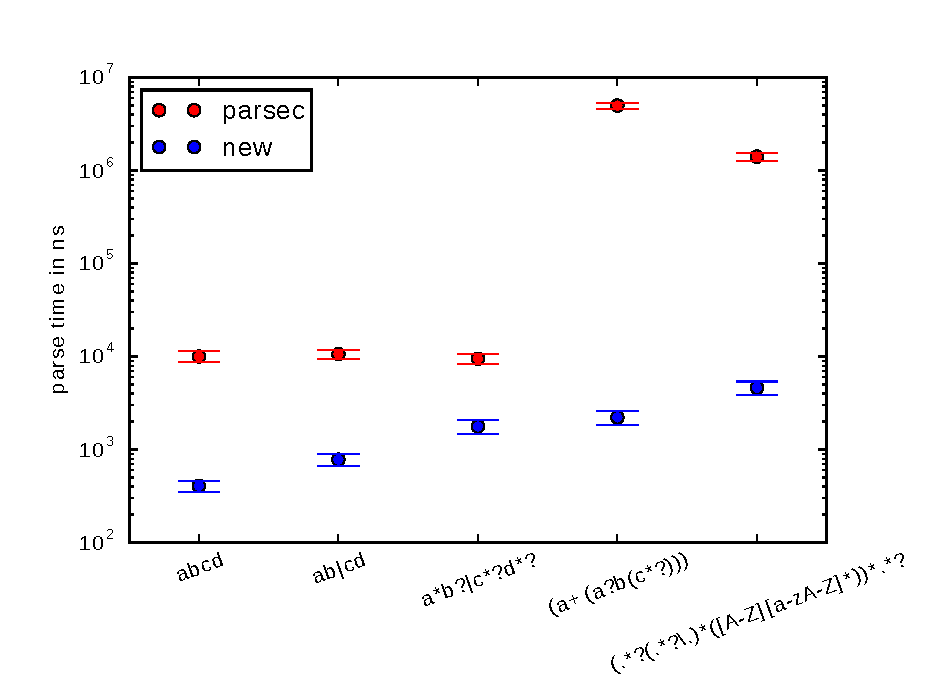
\includegraphics[width=\linewidth]{graphs/logplot-parserspeed-robust}

  \caption[Regular expression grammar parse time]{\figlabel{regex-syntax-parsing}Comparison of two ways of parsing the
regular expression syntax. Since the measurements are very noisy, the median
with the MAD (median absolute deviation) are plotted.}
\end{figure}

\chapter{Benchmark}
\seclabel{benchmarks}
All benchmarks were obtained using Google's
caliper\footnote{\url{https://code.google.com/p/caliper/}}, which
takes care of the most obvious benchmarking blunders.  It runs a
warm-up before measuring, runs all experiments in separate VMs,
helps circumvent dead-code detection by accepting the output of
dummy variables as input, and fails if compilation occurs during
experiment evaluation.  The source code of all benchmarks is
available, together with the sources of the project, on Github. We
ran all benchmarks on a 2.3 GHz, i7 Macbook Pro.

As we saw in \Secref{related}, there is a surprising dearth
of regular expression engines that can extract nested capture groups
-- never mind extracting entire parse trees -- that do not backtrack.
Back-tracking implementations are exponential in their run-time,
and so we see in \Figref{patho} (note the log plot) how the run-time
of ``java.util.regex'' quickly explodes exponentially, even for tiny input, for
a pathological regular expression, while our approach slows down
only linearly. The raw data is seen in \Tabref{patho}.

\begin{figure}[htp]
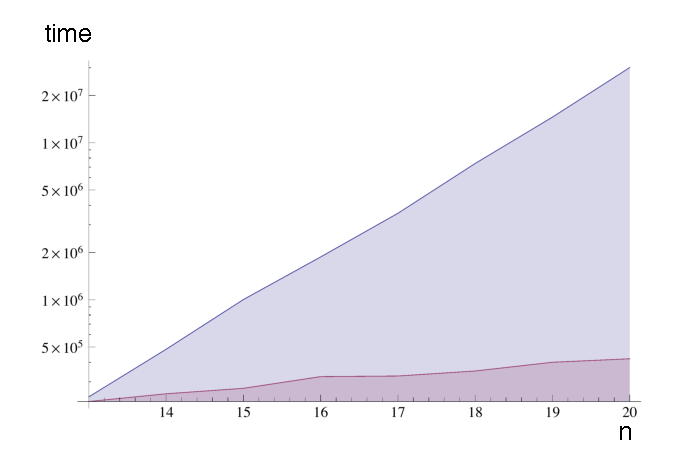
\includegraphics[width=\linewidth]{graphs/pathological-with-axes.pdf}
\caption[Pathological regular expression parse time]{Time in nanoseconds for matching $\textit{a?}^n\textit{a}^n$ against
input $\textit{a}^n$. Bottom (purple) line is our approach, top (blue) line is
java.util.regex.}
\figlabel{patho}
\end{figure}

\begin{table*}[htb]\center
\begin{tabular}{ccccccccc}
\toprule
$n$ & 13 & 14 & 15 & 16 & 17 & 18 & 19 & 20\tabularnewline
\midrule
java.util.regex & 241 & 484 & 1003 & 1874 & 3555 & 7381 & 14561 & 30116\tabularnewline
Ours & 225 & 252 & 273 & 32 & 327 & 352 & 400 & 421\tabularnewline
\bottomrule
\end{tabular}
\caption[Matching times $\textit{a?}^n\textit{a}^n$ against input $\textit{a}^n$.]{Matching times, in microseconds, for matching
  $\textit{a?}^n\textit{a}^n$ against input $\textit{a}^n$.}
\tablabel{patho}
\end{table*}

In the opposite case, in the case of a regular expression that's
crafted to prevent any back-tracking, java.util.regex outperforms
our approach by more than factor 2, as seen in \Tabref{abc} -- but
bear in mind that java.util.regex does not extract parse trees, but
only the last match of all capture groups.  A backtracking
implementation that actually does produce complete parse trees is
JParsec\footnote{\url{http://jparsec.codehaus.org}}, which, as also
seen in \Tabref{abc}, performs on par with our approach.

Note that because java.util.regex achieves its back-tracking through recursion,
we had to set the JVM's stack size to one Gigabyte for it to parse the input.
Since default stack size is only a few megabytes, this makes using
java.util.regex a security risk, even for unproblematic regular expressions
that cannot cause backtracking, since an attacker can potentially force the VM
to run out of stack space.

\begin{table}[htp]\center
\begin{tabular}{cc}
\toprule
Tool & Time\tabularnewline
\midrule
JParsec & 4,498\tabularnewline
java.util.regex & 1,992\tabularnewline
Ours & 5,332\tabularnewline
\bottomrule
\end{tabular}
\caption[Matching times regular expression \texttt{((a+b)+c)+} against input $(a^{200}bc)^{2000}$]{
  Matching regular expression \texttt{((a+b)+c)+} against input
$(a^{200}bc)^{2000}$, where $a^{200}$ denotes 200 times character `a'. Time in
microseconds.}
\tablabel{abc}
\end{table}

Finally, as a more realistic example, neither chosen to favor
back-tracking nor to avoid it,  extracts all class names, with their
package names, from the project sources itself.  As seen in
\Tabref{real}, our approach outperforms java.util.regex by 40\%,
even though our approach constructs the entire parse tree, and thus
all class names, while java.util.regex outputs only the last matched
class name. JParsec was not included in this experiment, since it does
not allow non-greedy matches. Even though it is possible to build
a parser that produces the same AST, it would necessarily look very
different (using negation) from the regular expression.

\begin{table}[htp]\center
\begin{tabular}{cc}
\toprule
Tool & Time\tabularnewline
\midrule
java.util.regex & 11,319\tabularnewline
Ours & 8,047\tabularnewline
\bottomrule
\end{tabular}
\caption[Matching times for finding all java class names]{Runtimes, in microseconds, for finding all java class names in all
  .java files in the project itself. The regular expression used is
  \texttt{(.*?([a-z]+\textbackslash.)*([A-Z][a-zA-Z]*))*.*?}.
Runtime in microseconds}
\tablabel{real}
\end{table}


\chapter{Conclusion}
Regular expression make for lightweight parsers and there are many cases
where data is extracted this way. If such data is structured
instead of flat, a parser that produces trees is superior to a standard
regular expression parser. We provide such an algorithm with modern
optimizations applied using results from persistent data-structures to avoid
unnecessary memory consumption and the slow-down that this would produce. 
This algorithm is able to provide the same semantics as backtracking, but 
without an exponential worst case.

Our approach can produce entire parse trees from matching regular expressions
in a single pass over the string and do so asymptotically no slower than
regular expression matching without any extraction.  The practical performance
is on par with traditional back-tracking solutions if no backtracking ever
happens, exponentially outperforms back-tracking approaches for pathological
input, and in a realistic scenario outperforms backtracking by 40\%, even
though our approach produces the full parse tree, and the backtracking
implementation doesn't. All source code and all benchmarks are available under
a free license on Github\cite{Schwarz:10861} at
\url{https://github.com/nes1983/tree-regex}.

\bibliographystyle{plain}
\bibliography{biblio}
\addcontentsline{toc}{chapter}{Bibliography}

\listoffigures
\listoftables
\listofalgorithms
\addcontentsline{toc}{chapter}{List of Algorithms}
\end{document}
